\documentclass{article}
\usepackage[T1]{fontenc}
\usepackage[utf8]{inputenc}
\usepackage[polish]{babel}
\usepackage{amsmath}
\usepackage{multirow}
\usepackage{listings}
\usepackage{listingsutf8}
\usepackage{longtable}
\usepackage{float}
\usepackage{graphicx}
\usepackage{caption}

%{Informatyka stosowana 2024, I st., semestr VI}

\lstset{
    inputencoding=utf8,
    extendedchars=true,
    literate=%
    {ą}{{\k{a}}}1
    {ć}{{\'c}}1
    {ę}{{\k{e}}}1
    {ł}{{\l{}}}1
    {ń}{{\'n}}1
    {ó}{{\'o}}1
    {ś}{{\'s}}1
    {ź}{{\'z}}1
    {ż}{{\.z}}1
    {Ą}{{\k{A}}}1
    {Ć}{{\'C}}1
    {Ę}{{\k{E}}}1
    {Ł}{{\L{}}}1
    {Ń}{{\'N}}1
    {Ó}{{\'O}}1
    {Ś}{{\'S}}1
    {Ź}{{\'Z}}1
    {Ż}{{\.Z}}1
}


\author{
	{Kacper Czernik 242371} \\
	{Mateusz Grzeszczak 242398}\\ 
{Prowadzący: Dr inż. Marcin Kacprowicz }
}

\title{Komputerowe systemy rozpoznawania 2023/2024\\Projekt 1. Klasyfikacja dokumentów tekstowych}
\begin{document}
\maketitle

\section{Cel projektu}
Celem projektu jest stworzenie aplikacji do klasyfikacji dokumentów tekstowych przy użyciu metody k-NN (k najbliższych sąsiadów) w technologii JDK. Aplikacja ma za zadanie ekstrahować cechy z tekstów oraz przeprowadzić klasyfikację tych posiadających etykiety: west-germany, usa, france, uk, canada, japan. Projekt ma uwzględniać analizę skuteczności klasyfikacji przy różnych wartościach parametru k, proporcjach podziału zbioru oraz zastosowanych metrykach i miarach podobieństwa tekstów, z uwzględnieniem miar jakości klasyfikacji.


\section{Klasyfikacja nadzorowana metodą $k$-NN.  Ekstrakcja cech, wektory cech}
Metoda k najbliższych sąsiadów (k-NN) jest powszechnie znanym algorytmem leniwym służącym do klasyfikacji nadzorowanej, który działa w myśl zasadzie "podobieństwo przyciąga". Dla nowego przypadku do klasyfikacji, algorytm identyfikuje k najbliższych sąsiadów według odległości od nowego przypadku. Nowy przypadek jest następnie klasyfikowany poprzez przyporządkowanie większościowe najbliższych sąsiadów. Odległość obliczana jest za pomocą wybranej uprzednio metryki.\\

\textbf{Parametry wejściowe:}
\begin{itemize}
    \item $k$: liczba najbliższych sąsiadów branych pod uwagę przy klasyfikacji.
    \item Zbiór treningowy: zbiór przypadków treningowych z etykietami klas, które są wykorzystywane do klasyfikacji nowych przypadków.
    \item Metryka odległości: funkcja określająca odległość pomiędzy przypadkami, np. metryka euklidesowa, metryka uliczna czy metryka Czebyszewa.
\end{itemize}

\textbf{Wyniki:}
\begin{itemize}
    \item Klasa, do której należy nowy przypadek, na podstawie głosowania sąsiadów.
    \item Stopień pewności klasyfikacji, np. proporcja głosów dla danej klasy.
\end{itemize}


\noindent W celu ekstrakcji cech charakterystycznych tekstu stworzony zostanie wektor cech, który opisuje tekst na podstawie następujących cech 10 cech, tu warto zaznaczyć że cechy 1-3 to wartości słownikowe a pozostałe (4-10) są czysto statystycznym ujęciem. Wektor ten wykorzystany zostanie w algorytmie kNN do obliczenia odległości między sąsiadami. \newline

\noindent W trakcie procesu ekstrakcji cech z tekstu, metoda wartości słownikowych zostanie zastosowana w celu wyłonienia kraju, dla którego odnotowano największą liczbę wystąpień. A wartość tej cechy wyliczana będzie przy pomocy poniższego wzoru:

\begin{equation}
    c = \frac{x}{T}
\end{equation}

Gdzie:
\begin{itemize}
    \item $c$ to wartość cechy.
    \item $x$ to liczba wystąpień słów dla najczęściej wspominanego państwa.
    \item $T$ to całkowita ilość wystąpień słów z danego słownika.
\end{itemize}

Wartości cech 4-5, 7-8 oraz 10 wyliczane będą przy pomocy poniższego wzoru:

\begin{equation}
    c = x
\end{equation}

Gdzie:
\begin{itemize}
    \item $c$ to wartość danej cechy.
    \item $x$ to ilość słów z tekstu spełniających zadane kryteria.
\end{itemize}

Wartość cechy 6 określana będzie przy pomocy następującego wzoru:

\begin{equation}
    c = x
\end{equation}

Gdzie: 
\begin{itemize}
    \item $c$ to wartość danej cechy.
    \item $x$ to całkowita ilość słów z danego tekstu.
\end{itemize}

Wartość cechy 9 określana będzie przy pomocy następującego wzoru:

\begin{equation}
    c = x
\end{equation}

Gdzie: 
\begin{itemize}
    \item $c$ to wartość danej cechy.
    \item $x$ to ilość znaków najdłuższego słowa.
\end{itemize}

Wybrane przez nas cechy zostały zaprezentowane poniżej:
\begin{enumerate}
    \item Liczba odniesień do prominentnych postaci politycznych z danego kraju, interpretowana za pomocą metody wartości słownikowej. Przygotowany do tego celu uwzględnia wybranych polityków od 1945 roku. Zliczane będą jedynie wystąpienia ich nazwisk. (patrz wzór (1)).
    \item Liczba wspomnień walut charakterystycznych dla danego kraju, wyrażona poprzez wartość słownikową. Pod uwagę wzięte zostają także nieoficjalne oraz skrótowe określenia tych walut, takie jak „dlr” dla dolara. (patrz wzór (1)).
    \item Liczba wystąpień pojęć nawiązujących do geografii danego kraju, rozpoznawanego przy pomocy uprzednio skonstruowanego słownika. W skład tego słownika wchodzą zarówno określenia nazw danego kraju, jak np. „U.S” bądź „USA” dla Ameryki, jak i nazwy niemieckich landów. (patrz wzór (1)).\newline

    Przykłady dla poniższych cech opisane zostaną przy pomocy przykładowego tekstu: „Sed ut perspiciatis, unde omnis iste natus error sit voluptatem accusantium” będącego wycinkiem „Loreum ipsum”. \newline

    \item Ilość słów rozpoczynających się wielką literą. Bazując na tekście przykładowym, możemy stwierdzić, że wartość tej cechy wynosić będzie 1, ponieważ jedynym słowem zaczynającym się z wielkiej litery jest „Sed”. (patrz wzór (2)).
    \item Ilość słów rozpoczynających się małą literą. Ponownie odnosząc się do tekstu przykładowego, możemy zaobserwować, że wartość tej cechy wynosić będzie 10. (patrz wzór (2)).
    \item Całkowita ilość słów. Jest to prawdopodobnie najprostsza do określenia cecha w naszym zestawieniu. Dla tekstu przykładowego jej wartość wynosić będzie 11. (patrz wzór (3)).
    \item Ilość słów o długości większej bądź równej 10 znaków. Przykładowe słowa pasujące do tej kategorii to „perspiciatis” oraz „accusantium”. (patrz wzór (2)).
    \item Ilość słów krótszych niż 5 lub równych 5 znaków. Słowami znajdującymi się w przykładowym tekście, mającymi mniej niż 5 znaków, są np.: „ut”, „error” bądź „sit”. (patrz wzór (2)).
    \item Ilość znaków w najdłuższym słowie. W przykładowym fragmencie „Loreum ipsum”, słowem które jest najdłuższe, jest słowo „perspiciatis”, które składa się z 13 znaków. (patrz wzór (4)).
    \item Ilość słów zawierających w sobie co najmniej jeden znak "\textendash", przykładem takiego słowa może być na przykład "politically-influential", w naszym tekście przykładowym nie znajduje się nawet jedno słowo spełniające to kryterium więc wartość tej cechy wynosiła by 0. (patrz wzór (3))
\end{enumerate}

Sam wektor prezentować się będzie w następujący sposób:
\[ V = [c_1,c_2,c_3, \ldots , c_9, c_{10}] \]


%==============================================================================================


\section{Miary jakości klasyfikacji}

W trakcie zadania wykorzystano standardowe miary jakości klasyfikacji, które są powszechnie stosowane w analizie wyników klasyfikatora. Zaprezentowane zostały krótkie opisy oraz konkretne wzory miar użytych w eksperymencie. Oznaczenia i objaśnienia symboli są jednolite dla wszystkich wzorów zawierających się poniżej.

\subsection*{Objaśnienia symboli:}
\begin{itemize}

    \item \textbf{TP (True Positives)} = Poprawna klasyfikacja pozytywnych przypadków: Liczba przypadków, w których klasyfikator poprawnie przypisał artykuł do klasy.
    
    \item \textbf{TN (True Negatives)} = Poprawna klasyfikacja negatywnych przypadków: Liczba przypadków, w których klasyfikator poprawnie sklasyfikował artykuł jako nie należący do klasy.
    
    \item \textbf{FP (False Positives)} = Błędna klasyfikacja pozytywnych przypadków: Liczba przypadków, w których klasyfikator błędnie sklasyfikował artykuł, uznał on że artykuł należy do klasy a w rzeczywistości nie należy.
    
    \item \textbf{FN (False Negatives)} = Błędna klasyfikacja negatywnych przypadków: Liczba przypadków, w których klasyfikator błędnie sklasyfikował artykuł jako nie należący do klasy, a w rzeczywistości powinien on być zaklasyfikowany jako należący.
    
    \item \textbf{Populacja}: przez populację rozumiemy wszystkie występujące wyrażenia (\textbf{TP + TN + FP + FN}).
\end{itemize}

\subsection*{wykorzystane miary:} 

Analiza wydajności klasyfikatora stanowi kluczowy etap w przetwarzaniu danych. Miary takie jak precyzja, czułość i F1 są niezbędne do zrozumienia, jak dobrze klasyfikator radzi sobie z identyfikacją właściwych klas. W przeciwieństwie do tych miar, ocena dokładności jest wyliczana jednorazowo dla całego zbioru danych, a nie dla poszczególnych klas. Stosujemy te miary, aby dokładnie ocenić skuteczność naszych modeli w identyfikowaniu pozytywnych przypadków i minimalizacji błędów.\newline

\noindent Wartości tych miar mieszczą się w przedziale od 0 do 1, gdzie 0 oznacza najgorszą możliwą wydajność klasyfikatora, a 1 - najlepszą. Wartości bliższe 1 oznaczają lepszą wydajność klasyfikatora, podczas gdy wartości bliższe 0 sugerują gorszą wydajność.



\subsubsection*{Dokładność (Accuracy)}
 
Jest to stosunek liczby poprawnie sklasyfikowanych dokumentów (TP + TN) do liczby wszystkich dokumentów w zbiorze testowym. Wyraża się wzorem: \newline
 
\begin{equation}
    \text{Accuracy} = \frac{TP + TN}{\text{populacja}}
\end{equation}


\noindent Głównym celem dokładności jest mierzenie ogólnej skuteczności klasyfikatora w poprawnym identyfikowaniu zarówno pozytywnych, jak i negatywnych przypadków w zbiorze danych. Jednakże, należy pamiętać, że w przypadku niezrównoważonych zbiorów danych, gdzie jedna klasa może dominować nad innymi, accuracy może być mylącym miernikiem. \newline 

\noindent Przykładem, w którym mara dokładności może zakłamywać wynik może być następująca sytuacja: \newline

\noindent Załóżmy że mamy 1000 dokumentów, z czego 800 pochodzi z UK, a 200 z West-Germany, i klasyfikator poprawnie przypisał 780 dokumentów do UK jako TP i 100 dokumentów z West-Germany jako TN, to otrzymujemy Accuracy równą 0.88, co oznacza, że poprawnie zostało sklasyfikowanych 88\% dokumentów. Jednakże, kiedy przyjrzymy się tej sytuacji bliżej, zauważymy, że klasa UK jest rozpoznawana w 97.50\%, natomiast klasa West-Germany tylko w 50\%.

\subsubsection*{Precyzja (Precision)}

Określa stosunek liczby prawdziwie pozytywnych przypadków (TP) do sumy prawdziwie pozytywnych i fałszywie pozytywnych przypadków (FP). Wzór na precyzję to: \newline
 
\begin{equation}
    \text{Precision} = \frac{TP}{TP + FP}
\end{equation}

\noindent Korzystając z precyzji, możemy odpowiedzieć na pytanie: "Z wszystkich przypadków sklasyfikowanych jako pozytywne, ile z nich faktycznie jest pozytywnych?", przedstawia ona dokładność w rozpoznawaniu klas. \newline

\noindent W momencie kiedy chcemy obliczyć precyzję dla całego zbioru a nie tylko dla jednej klasy możemy wykorzystać średnią ważoną zgodnie z poniższym wzorem:

\begin{equation}
    Precision_c = \frac{\sum_{i=1}^{n} Precision_i \times TP_i}{\sum_{i=1}^{n} TP_i}
\end{equation}

\noindent gdzie: \\
$Precision_c$ jest precyzją dla całego procesu klasyfikacji.

\subsubsection*{Czułość (Recall)}

Jest to stosunek liczby prawdziwie pozytywnych przypadków (TP) do sumy prawdziwie pozytywnych i fałszywie negatywnych przypadków (FN). Wzór na czułość to: \newline

\begin{equation}
    \text{Recall} = \frac{TP}{TP + FN}
\end{equation}


\noindent Czułość jest miarą, która ocenia zdolność klasyfikatora do identyfikowania wszystkich rzeczywiście pozytywnych przypadków w zbiorze danych. To oznacza, w jakim stopniu klasyfikator radzi sobie z wykrywaniem przypadków, które faktycznie należą do badanej klasy, czyli mówiąc prościej ile z pozytywnych zostało właściwie wykrytych. \newline

\noindent Wzór dla czułości dla całego procesu klasyfikacji wygląda następująco:

\begin{equation}
    Recall_c = \frac{\sum_{i=1}^{n} Recall_i \times TP_i}{\sum_{i=1}^{n} TP_i}
\end{equation}

\noindent gdzie: \\
$Recall_c$ jest czułość dla całego procesu klasyfikacji.

\subsubsection*{Miara F1}

Miara F1 to średnia harmoniczna miar Precision i Recall. Oblicza się ją według wzoru: \newline
 
\begin{equation}
    \text{F1} = 2 \times \frac{\text{Precision} \times \text{Recall}}{\text{Precision} + \text{Recall}}
\end{equation}


\noindent Korzystamy z miary F1, ponieważ pozwala ona na ocenę wydajności klasyfikatora w sposób, który uwzględnia zarówno jego zdolność do poprawnego identyfikowania pozytywnych przypadków, jak i ograniczanie błędów, co daje bardziej kompleksową ocenę niż każda z tych miar osobno. \newline

\noindent wartość dla całego procesu klasyfikacji obliczana jest jako średnia harmoniczna ogólnego precision i ogólnego recall

\begin{equation}
    F1_c = 2 \times \frac{Precision_c \times Recall_c}{Precision_c + Recall_c}
\end{equation}

\noindent gdzie: \\
$F_c$ jest wartością miary F1 dla całego procesu klasyfikacji.
%==========


\subsection*{Analiza Wydajności Klasyfikatora}

W tej sekcji przeprowadzimy analizę wydajności klasyfikatora dla zbioru danych składającego się z trzech klas: Japan, USA i Canada. Rozpoczniemy od przedstawienia macierzy pomyłek oraz obliczenia dokładności.


\subsubsection*{Tabela z Danymi i Obliczeniami Dokładności}

\begin{table}[htbp]
\centering
\caption{Macierz Pomyłek dla Klasyfikacji 3 Przykładowych Krajów oraz Obliczenia Dokładności \newline} 
\label{tab:data_accuracy}
\begin{tabular}{|c|c|c|c|}
\hline
Zaklasyfikowany \ Rzeczywisty kraj & Japan & USA & Canada \\ \hline
Japan                              & 90    & 10  & 20     \\ \hline
USA                                & 25    & 85  & 25     \\ \hline
Canada                             & 30    & 25  & 80     \\ \hline
\end{tabular}
\end{table}

\noindent wykonujemy następujące podstawienia działając z perspektywy klasy Japan: \\

\noindent Liczba tekstów prawdziwie pozytywnie zaklasyfikowanych do Japan: TP = 90 \\
Liczba tekstów prawdziwie negatywnie zaklasyfikowanych do Japan: TN = 215 \\
Liczba tekstów fałszywie pozytywnie zaklasyfikowanych do Japan: FP = 30 \\
Liczba tekstów fałszywie negatywnie zaklasyfikowanych do Japan: FN = 55 \\


\begin{equation}
    \text{Dokładność:} \frac{90 + 215}{90 + 215 + 30 + 55} = \frac{305}{390} \approx 0.78.
\end{equation}

\subsubsection*{Obliczenia dla Precyzji, Czułości i F1-score}

Dla każdej klasy (Japan, USA, Canada) obliczamy precyzję (Precision), czułość (Recall) i miarę F1 wykorzystując do tego wzory (6,8,10) wymienione w powyższej sekcji: \\

\subsubsection*{Dla klasy Japan:}

\begin{equation}
    \text{Precyzja (Precision): } \frac{90}{90 + 25 + 30} \approx 0.64
\end{equation}
\begin{equation}
    \text{Czułość (Recall): } \frac{90}{90 + 10 + 20} \approx 0.75
\end{equation}
\begin{equation}
    \text{F1-score: } 2 \times \frac{0.64 \times 0.75}{0.64 + 0.75} \approx 0.69
\end{equation}

\subsubsection*{Dla klasy USA:}

\begin{equation}
    \text{Precyzja (Precision): } \frac{85}{85 + 10 + 25} \approx 0.71
\end{equation}
\begin{equation}
    \text{Czułość (Recall): } \frac{85}{85 + 25 + 25} \approx 0.62
\end{equation}
\begin{equation}
    \text{F1-score: } 2 \times \frac{0.71 \times 0.62}{0.71 + 0.62} \approx 0.66
\end{equation}

\subsubsection*{Dla klasy Canada:}

\begin{equation}
    \text{Precyzja (Precision): } \frac{80}{80 + 20 + 25} \approx 0.67
\end{equation}
\begin{equation}
    \text{Czułość (Recall): } \frac{80}{80 + 30 + 25} \approx 0.62
\end{equation}
\begin{equation}
    \text{F1-score: } 2 \times \frac{0.67 \times 0.62}{0.67 + 0.62} \approx 0.64
\end{equation}


\subsubsection*{Tabela Podsumowująca Miary Jakości Klasyfikacji dla Każdego Kraju}

Poniższa tabela podsumowuje miary jakości klasyfikacji dla każdego kraju, włączając dokładność, precyzję, czułość oraz miarę F1.


\begin{table}[htbp]
\centering
\caption{Tabela Podsumowująca Miary Jakości Klasyfikacji dla Każdego Kraju \newline}
\label{tab:summary_metrics}
\begin{tabular}{|c|c|c|c|c|}
\hline
Kraj    & Dokładność & Precyzja & Czułość & F1-score \\ \hline
Japonia & 0.78       & 0.64     & 0.75    & 0.69     \\ \hline
USA     & 0.78       & 0.71     & 0.62    & 0.66     \\ \hline
Kanada  & 0.78       & 0.67     & 0.62    & 0.64     \\ \hline
\end{tabular}
\end{table}

\subsubsection*{Obliczenia dla Precyzji, Czułości i F1-score dla całego procesu klasyfikacji}

Wykorzystując uzyskane wcześniej wyniki w celu uzyskania miar czułości, precyzji oraz F1 dla całego procesu klasyfikacji, wykorzystamy do tego celu wymienione wcześniej wzory (7,9,11):

\subsubsection*{precyzja dla całego procesu klasyfikacji}
\begin{equation}
    Precision_c = \frac{0.64 \times 90 + 0.71 \times 85 + 0.67 \times 80}{90 + 85 + 80} = \frac{57.6 + 60.35 + 53.6}{255} \approx 0.67 
\end{equation}

\subsubsection*{czułość dla całego procesu klasyfikacji}
\begin{equation}
    Recall_c = \frac{0.75 \times 90 + 0.62 \times 85 + 0.62 \times 80}{90 + 85 + 80} = \frac{67.5 + 52.7 + 49.6}{255} \approx 0.66
\end{equation}

\subsubsection*{miara F1 dla całego procesu klasyfikacji}
\begin{equation}
    F1_c = 2 \times \frac{0.67 \times 0.66}{0.67 + 0.66} \approx 0.66
\end{equation}

\subsubsection*{Interpretacja Wyników}

Dokładność (Accuracy): Poziom dokładności dla wymienionych krajów wynosi w przybliżeniu 0.78. Oznacza to, że klasyfikator radzi sobie stosunkowo dobrze ze wszystkimi klasami.\\

\noindent Precyzja (Precision): Dla każdego kraju precyzja waha się w granicach od około 0.64 do 0.71. Wyższa precyzja oznacza, że mniej dokumentów jest fałszywie zaklasyfikowanych jako należące do danej klasy.
\begin{itemize}
    \item Analizując konkretny przypadek dla kraju Japan, dla którego wartość precyzji wyniosła 0.64, możemy to zinterpretować jako fakt że 64\% dokumentów rozpoznanych jako należące do klasy japan rzeczywiście do niej należy a 36\% nie należy.\\
\end{itemize}

\noindent Czułość (Recall): Czułość dla każdego kraju również oscyluje w granicach od około 0.62 do 0.75. Wyższa czułość oznacza, że więcej faktycznie pozytywnych przypadków zostało wykrytych przez klasyfikator.
\begin{itemize}
    \item Ponownie analizując przypadek dla kraju Japan, dla którego wartość miary czułości wynosi 0.75, co oznacza, że ze wszystkich pozytywnych dokumentów klasyfikator poprawnie wykrył 75\% pozytywnych dokumentów, a zaledwie 25\% zaklasyfikował do błędnej klasy. \\
\end{itemize}

\noindent F1-score: Wartości F1-score dla każdego kraju wahają się od około 0.64 do 0.69. Im wyższa wartość F1-score, tym lepiej klasyfikator radzi sobie z równowagą między precyzją a czułością.
\begin{itemize}
    \item Ostatni już raz przyglądając się klasie Japan. Miara F1 dla tego kraju wyniosła 0.69 tak więc możemy mówić że klasyfikator osiągnął umiarkowaną precyzję oraz czułość, czyli większa ilość elementów została poprawnie przypisana do klasy (TP), a mniejsza ilość elementów została przypisana do błędnej klasy (FP oraz FN) i można uznać, że algorytm działa relatywnie poprawnie.
\end{itemize}

\noindent Ogólnie rzecz ujmując, mamy do czynienia z równowagą między precyzją a czułością dla wszystkich klas, co sugeruje, że klasyfikator działa w miarę skutecznie dla wszystkich trzech krajów wziętych pod uwagę w przykładzie.\\

\noindent Dodatkowo analiza miary dla całego procesu klasyfikacji jesteśmy w stanie poddać ocenie skuteczność całego modelu klasyfikacyjnego co może dostarczyć dodatkowych informacji, które mogą być trudniejsze do wyodrębnienia z miar dla pojedynczych klas, bądź mogą dostarczyć te informacje bez potrzeby ręcznego analizowania wyników dla każdej z  klas z osobna.



%==============================================================================================



\section{Metryki i miary podobieństwa tekstów w klasyfikacji}


W kontekście klasyfikacji tekstów, mierzymy odległości między wektorami cech, które reprezentują teksty. Metryki są narzędziami matematycznymi, które pozwalają nam określić, jak bardzo dwa wektory cech różnią się od siebie lub są do siebie podobne. Te odległości są istotne, ponieważ na ich podstawie algorytmy klasyfikacji podejmują decyzje dotyczące przypisania nowego tekstu do odpowiedniej klasy.\newline

\noindent Definicja metryki w tym kontekście zakłada, że dla dowolnych dwóch wektorów cech, metryka określa odległość między nimi, która zawsze jest nieujemna, a równa zero tylko wtedy, gdy wektory są identyczne. Metryki są symetryczne, co oznacza, że odległość między wektorem cech A i wektorem cech B jest taka sama jak odległość między wektorem cech B i wektorem cech A. \newline

\subsection*{wykorzystane metryki}

\subsubsection*{metryka Euklidesowa}

Metryka euklidesowa jest jedną z najbardziej powszechnie stosowanych metryk w analizie danych. Definicja metryki euklidesowej jest prosta i intuicyjna. Dla dwóch punktów w przestrzeni cech, odległość euklidesowa między nimi jest długością prostej linii łączącej te punkty. Matematycznie, dla dwóch wektorów cech a i b o wymiarach n, odległość euklidesowa jest określona jako pierwiastek kwadratowy z sumy kwadratów różnic między odpowiadającymi elementami tych wektorów. Metryka euklidesowa określana jest następującym wzorem: \newline

\begin{equation}
   d(\mathbf{a}, \mathbf{b}) = \sqrt{\sum_{i=1}^{n} (a_i - b_i)^2}
\end{equation}

\subsubsection*{metryka uliczna}

Metryka uliczna, znana również jako metryka Manhattan, to jedna z podstawowych metryk używanych w analizie odległości. Dla dwóch punktów \\ $\mathbf{a} = (a_1, a_2, ..., a_n)$ i $\mathbf{b} = (b_1, b_2, ..., b_n)$ w przestrzeni $n$-wymiarowej, odległość między nimi za pomocą metryki ulicznej można obliczyć jako suma bezwzględnych różnic ich współrzędnych:

\begin{equation} d(\mathbf{a}, \mathbf{b}) = \sum_{i=1}^{n} |a_i - b_i| \quad(10) \end{equation}

\noindent W przestrzeni dwuwymiarowej (dla $n = 2$), metryka uliczna odpowiada długości najkrótszej ścieżki między dwoma punktami wzdłuż siatki ulic, gdzie można poruszać się tylko w kierunkach pionowych i poziomych. Miasto spełniające to takie kryteria istnieje w rzeczywistości i jest to Barcelona. \newline




\subsubsection*{metryka Czebyszewa}

Metryka ta oblicza odległość między dwoma punktami poprzez znalezienie największej różnicy między ich współrzędnymi. \newline

\noindent Dla dwóch punktów $\mathbf{a} = (a_1, a_2, ..., a_n)$ i $\mathbf{b} = (b_1, b_2, ..., b_n)$ w przestrzeni $n$-wymiarowej, odległość między nimi za pomocą metryki Czebyszewa można obliczyć jako maksimum bezwzględnych różnic ich współrzędnych:

\begin{equation} d(\mathbf{a},\mathbf{b}) = \max_{i=1}^{n} |a_i - b_i| \end{equation}

\noindent W metryce Czebyszewa odległość między dwoma punktami jest równa maksymalnej różnicy między ich współrzędnymi w każdym wymiarze. W praktyce oznacza to, że liczba wymiarów $n$ powinna być równa liczbie cech wektorów, które są brane pod uwagę w analizie odległości. \newline



\subsection*{miara podobieństwa tekstów}

\subsubsection*{uogólniona metoda n-gramów}

Nasze zadanie wymaga porównywania wektorów cech, gdzie niektóre z tych cech są reprezentowane przez wartości tekstowe, co uniemożliwia bezpośrednie zastosowanie standardowych metryk opartych na liczbach. Konieczne jest zatem użycie specjalnych miar podobieństwa tekstów do porównania tych wektorów, aby uzyskać adekwatne wyniki analizy. Znanych jest wiele miar pozwalających na osiągnięcie tego celu jednakże podczas realizacji zadania zdecydowaliśmy się na zastosowanie uogólnionej metody n-gramów znanej róznież jako metoda Niewiadomskiego. Metoda ta opisywania jest poniższym wzorem:

\begin{equation}
\mu_N(s_1, s_2) = \frac{2}{N^2 + N} \sum_{i=1}^{N(s_1)} \sum_{j=1}^{N(s_1)-i+1} h(i, j)
\end{equation}

gdzie:

\begin{itemize}
    \item \( h(i, j) \) przyjmuje wartość 1, jeśli i-elementowy podciąg w słowie \( s_1 \) zaczynający się od j-tej pozycji w słowie \( s_1 \) pojawia się przynajmniej raz w słowie \( s_2 \) (w przeciwnym razie \( h(i, j) = 0 \)),
    \item \( N(s_1) \) i \( N(s_2) \) to ilość liter w słowach \( s_1 \) i \( s_2 \),
    \item \( N = \max\{N(s_1), N(s_2)\} \),
    \item \( N^2 + N \) to ilość możliwych podciągów od 1-elementowych do N-elementowych w słowie o długości N.
\end{itemize}

\noindent Ważną rzeczą którą należy wspomnieć podczas omawiania uogólnionej miary n-gramów jest fakt że miara ta nie jest symetryczna, własność tą możemy jednak zniwelować korzystając z poniższego wzoru:

\begin{equation}
    \mu_{N_{\text{sym}}}(s_1, s_2) = \min\{\mu_N (s_1, s_2), \mu_N (s_2, s_1)\}
\end{equation}

\subsubsection*{n-gramy}

N-gramy są to sekwencje n kolejnych elementów w tekście lub ciągu danych, gdzie elementami mogą być litery, słowa, czy też inne znaki. \newline

\noindent W kontekście analizy tekstu, n-gramy są używane do wyodrębnienia kontekstu lub struktury tekstu poprzez uwzględnienie sekwencji kolejnych elementów. Przykładami n-gramów to: trigramy (n=3), bigramy (n=2) oraz unigramy (n=1). \newline

Przykład dla słowa "Koteczek":
\begin{itemize}
    \item Unigramy: "K", "o", "t", "e", "c", "z", "e", "k".
    \item Bigramy: "Ko", "ot", "te", "ec", "cz", "ze", "ek".
    \item Trigramy: "Kot", "ote", "tec", "ecz", "cze", "zek".
\end{itemize}

\subsubsection*{odległość a podobieństwo}

W celu wykorzystania miary podobieństwa podczas pracy z metrykami musimy wyznaczyć odległość między porównywanymi słowami, do tego celu możemy wykorzystać poniższy wzór:

\begin{equation}
    d(s_1, s_2) = 1 - \mu_{N_{\text{sym}}}(s_1, s_2)
\end{equation}

\subsection*{Przykładowe zastosowanie metryk}

Aby zilustrować działanie omawianych wcześniej metryk, poniżej przedstawiono przykładowe obliczenia dla dwóch wektorów:

\[ v_1 = [0.21, 5, 0.98, \text{kot}] \]
\[ v_2 = [0.13, 12, 0.99, \text{kotek}] \]

\noindent Wektory te są używane do demonstracji działania metryk w kontekście porównywania tekstowych wartości cech.

\subsection*{Wykorzystanie uogólnionej miary n-gramów}

Już na pierwszy rzut oka widać, że nasze wektory \( \mathbf{v}_1 \) i \( \mathbf{v}_2 \) nie są możliwe do bezpośredniego porównania ze względu na występowanie w nich wartości tekstowych. Możemy jednak wykorzystać w tym celu wspomnianą wcześniej uogólnioną miarę n-gramów. \newline

Słowo "kot" można podzielić na następujące n-gramy:

\begin{align*}
    n &= 1:  ["k", "o", "t"] \\
    n &= 2:  ["ko", "ot"] \\
    n &= 3:  ["kot"]
\end{align*}


Słowo "kotek" można podzielić na następujące n-gramy:
\begin{align*}
    n &= 1:  ["k", "o", "t", "e", "k"] \\
    n &= 2:  ["ko", "ot", "te", "ek"] \\
    n &= 3:  ["kot", "ote", "tek"] \\
    n &= 4:  ["kote", "otek"] \\
    n &= 5:  ["kotek"]
\end{align*}

\subsubsection*{obliczanie \( \mu_N(("\text{kotek}"), ("\text{kot}")) \)}

\noindent Dla uproszczenia podstawień do wzoru (28) wyliczamy uprzednio następujące wartości 


\[  N("\text{kot}") = 3 \]
\[ N("\text{kotek}") = 5 \]
\[ N = \max\{3, 5\} = 5 \]
\[ N^2 + N = 5^2 + 5 = 25 + 5 = 30 \]



\noindent ostateczny wzór (28) z podstawionymi wartościami wyliczonymi powyżej:

\begin{equation}
    \mu_N(("\text{kotek}"), ("\text{kot}")) = \frac{2}{30} \sum_{i=1}^{5} \sum_{j=1}^{5-i+1} h(i, j)
\end{equation}

\noindent Przyjrzyjmy się krok po kroku obliczeniom: \newline

\noindent Dla \( i = 1 \) (1-gramy):
\begin{align*}
    h(1, 1) &= 1 & \text{(n-gram "k" występuje w obu słowach)} \\
    h(1, 2) &= 1 & \text{(n-gram "o" występuje w obu słowach)} \\
    h(1, 3) &= 1 & \text{(n-gram "t" występuje w obu słowach)} \\
    h(1, 4) &= 0 & \text{(brak n-gramu na tej pozycji w jednym ze słów)} \\
    h(1, 5) &= 1 & \text{(n-gram "k" występuje w obu słowach))}
\end{align*}
Suma dla \( i = 1 \):
\begin{equation}
\sum_{j=1}^{5-1+1} h(1, j) = h(1, 1) + h(1, 2) + h(1, 3) + h(1, 4) + h(1, 5) = 4
\end{equation}

\noindent Dla \( i = 2 \) (2-gramy):
\begin{align*}
    h(2, 1) &= 0 & \text{(brak n-gramu na tej pozycji w jednym ze słów)} \\
    h(2, 2) &= 1 & \text{(n-gram "ko" występuje w obu słowach)} \\
    h(2, 3) &= 1 & \text{(n-gram "ot" występuje w obu słowach)} \\
    h(2, 4) &= 0 & \text{(brak n-gramu na tej pozycji w jednym ze słów)}
\end{align*}
Suma dla \( i = 2 \):
\begin{equation}
\sum_{j=1}^{5-2+1} h(2, j) = h(2, 1) + h(2, 2) + h(2, 3) + h(2, 4) = 2
\end{equation}

\noindent Dla \( i = 3 \) (3-gramy):
\begin{align*}
    h(3, 1) &= 0 & \text{(brak n-gramu na tej pozycji w jednym ze słów)} \\
    h(3, 2) &= 0 & \text{(brak n-gramu na tej pozycji w jednym ze słów)} \\
    h(3, 3) &= 1 & \text{(n-gram "kot" występuje w obu słowach)}
\end{align*}
Suma dla \( i = 3 \):
\begin{equation}
\sum_{j=1}^{5-3+1} h(3, j) = h(3, 1) + h(3, 2) + h(3, 3) = 1
\end{equation}

\noindent Dla \( i = 4 \) (4-gramy):
\begin{align*}
    h(4, 1) &= 0 & \text{(brak n-gramu na tej pozycji w jednym ze słów)} \\
    h(4, 2) &= 0 & \text{(brak n-gramu na tej pozycji w jednym ze słów)} \\
    h(4, 3) &= 0 & \text{(brak n-gramu na tej pozycji w jednym ze słów)}
\end{align*}
Suma dla \( i = 4 \):
\begin{equation}
\sum_{j=1}^{5-4+1} h(4, j) = h(4, 1) + h(4, 2) + h(4, 3) = 0
\end{equation}

\noindent Dla \( i = 5 \) (5-gramy):
\begin{align*}
    h(5, 1) &= 0 & \text{(brak n-gramu na tej pozycji w jednym ze słów)}
\end{align*}
Suma dla \( i = 5 \):
\begin{equation}
\sum_{j=1}^{5-5+1} h(5, j) = h(5, 1) = 0
\end{equation}


\noindent Kolejne kroki wyliczeń przedstawione zostały poniżej w celu łatwiejszej interpretacji. \newline

Dla $n = 1$:
\begin{equation}
    \mu_N(("\text{kotek}"), ("\text{kot}")) = \frac{2}{30} (4) = 0.2668
\end{equation}

Dla $n = 2$:
\begin{equation}
    \mu_N(("\text{kotek}"), ("\text{kot}")) = \frac{2}{30} (2) = 0.1334
\end{equation}

Dla $n = 3$:
\begin{equation}
    \mu_N(("\text{kotek}"), ("\text{kot}")) = \frac{2}{30} (1) = 0.0667
\end{equation}

Dla $n = 4$:
\begin{equation}
    \mu_N(("\text{kotek}"), ("\text{kot}")) = \frac{2}{30} (0) = 0
\end{equation}

Dla $n = 5$:
\begin{equation}
    \mu_N(("\text{kotek}"), ("\text{kot}")) = \frac{2}{30} (0) = 0
\end{equation}

\noindent Wartości miary n-gramów dla różnych wartości \( n \) pokazują, jak zmienia się podobieństwo między słowami "kot" i "kotek" w zależności od długości podciągów branych pod uwagę. Na podstawie tych wyników możemy stwierdzić, że dla \( n = 1 \) miara n-gramów daje największe podobieństwo między słowami, jednakowoż jako że pod uwagę bierzemy uogólnioną miarę ostateczny wynik wygląda następująco:


\begin{equation}
\mu_N(("\text{kotek}"), ("\text{kot}")) = \frac{2}{30} (7) = \frac{14}{30} = 0.4668
\end{equation}

\noindent Ostatecznie wartość uogólnionej miary n-gramów \( \mu_N("\text{kotek}"), ("\text{kot}") \) wynosi 0.4668, co wskazuje na pewne podobieństwo między słowami "kotek" i "kot". \newline


\subsubsection*{obliczanie \( \mu_N(("\text{kot}"), ("\text{kotek}")) \)}

\noindent Jako że miara Niewiadomskiego nie jest symetryczna, w celu uzyskania adekwatnego wyniku należy skorzystać ze wzoru (29). Oznacza to, że samo obliczenie \( \mu_N("\text{kotek}")("\text{kot}") \) nie wystarczy. Musimy również obliczyć wartość \( \mu_N("\text{kot}"), ("\text{kotek}") \). \newline

\noindent Podonie jak przy obliczaniu \( \mu_N("\text{kot}"), ("\text{kotek}") \) wykonujemy następujące podstawienia do wzoru (28):

\begin{equation}
    \mu_N(("\text{kot}"), ("\text{kotek}")) = \frac{2}{30} \sum_{i=1}^{3} \sum_{j=1}^{3-i+1} h(i, j)
\end{equation}

\noindent Kolejne kroki wyliczeń przedstawione zostały poniżej: \newline

Dla $n = 1$:
\begin{equation}
    \mu_N(("\text{kot}"), ("\text{kotek}")) = \frac{2}{30} (3) = 0.2001
\end{equation}

Dla $n = 2$:
\begin{equation}
    \mu_N(("\text{kot}"), ("\text{kotek}")) = \frac{2}{30} (2) = 0.1334
\end{equation}

Dla $n = 3$:
\begin{equation}
    \mu_N(("\text{kot}"), ("\text{kotek}")) = \frac{2}{30} (1) = 0.0667
\end{equation}

\noindent Ostatecznie wartość uogólnionej miary n-gramów \( \mu_N(("\text{kot}"), ("\text{kotek}")) \) wynosi 0.4668, co wskazuje na pewne podobieństwo między słowami "kot" i "kotek". \newline

\begin{equation}
    \mu_N(("\text{kot}"), ("\text{kotek}")) = \frac{2}{30} (6) = \frac{12}{30} = 0.4002
\end{equation}

\subsubsection*{}

\noindent W celu zniwelowania nie symetryczności miary Niewiadomskiego podstawiamy otrzymane wyniki pod wzór (29).


\begin{equation} \label{eq1}
\begin{split}
\mu_{N_{\text{sym}}}(&("\text{kot}"), ("\text{kotek}")) = \\
& = \min\{\mu_N (("\text{kot}"), ("\text{kotek}")), \mu_N (("\text{kotek}"), ("\text{kot}"))\} = \\
& = \min\{(0.4002), (0.4668)\} = 0.4002
\end{split}
\end{equation}





\subsection*{obliczanie odległości przy użyciu metryk}

\subsubsection*{podstawienia}

\noindent Podczas pracy na metrykach korzystać będziemy z następujących podstawień, wszystkie wartości pochodzą z wektorów \(v_1\) oraz \(v_2\) zaprezentowanych na początku tej sekcji. Wartości te są tożsame dla każdej z metryk. \newline

\noindent W celu obliczania odległości między słowami "kot" i "kotek" wykożystamy wzór (30). \newline

\begin{equation}
    d(("\text{kot}"), ("\text{kotek}")) = 1 - 0.4002 = 0.5998
\end{equation}

\noindent Podstawienia:
\begin{align*}
a_1 &= 0.21 & b_1 &= 0.13 \\
a_2 &= 5 & b_2 &= 12 \\
a_3 &= 0.98 & b_3 &= 0.99 
\end{align*}
\[ d(a_4, b_4) = d(("\text{kot}"), ("\text{kotek}")) = 0.5998\]



\subsubsection*{Metryka Euklidesowa}

Obliczmy odległość między \( v_1 \) i \( v_2 \) za pomocą metryki euklidesowej. (wzór 25) \newline

Obliczenia:
\begin{equation}
\begin{split}
d(v_1, v_2) &= \sqrt{(0.21 - 0.13)^2 + (5 - 12)^2 + (0.98 - 0.99)^2 + (0.5998)^2} \\
&= \sqrt{(0.08)^2 + (-7)^2 + (-0.01)^2 + 0.5998^2} \\
&= \sqrt{0.0064 + 49 + 0.0001 + 0.3597} \\
&\approx \sqrt{49.3663} \\
&\approx  7.0026
\end{split}
\end{equation}


\subsubsection*{Metryka Uliczna}

Obliczmy odległość między \( v_1 \) i \( v_2 \) za pomocą metryki ulicznej. (wzór 26) \newline

Obliczenia:
\begin{equation}
\begin{split}
d(v_1, v_2) &= |0.21 - 0.13| + |5 - 12| + |0.98 - 0.99| + |0.5998| \\
&= 0.08 + 7 + 0.01 + 0.5998 \\
&= 7.6898
\end{split}
\end{equation}


\subsubsection*{Metryka Czebyszewa}

Obliczmy odległość między \( v_1 \) i \( v_2 \) za pomocą metryki Czebyszewa. (wzór 27) \newline


Obliczenia:
\begin{equation}
\begin{split}
d(v_1, v_2) &= \max\{|0.21 - 0.13|, |5 - 12|, |0.98 - 0.99|, |0.5998|\} \\
&= \max\{0.08, 7, 0.01, 0.5998\} \\
&= 7
\end{split}
\end{equation}

\subsection*{Podsumowanie}

Ostateczny wynik (ten otrzymany po zniwelowaniu niesymetryczności przy pomocy wzoru (29)) uogólnionej miary n-gramów wyniósł 0.4002, co sugeruje, że słowa "kot" i "kotek" są dość podobne. \newline

\noindent Dodatkowo, zauważyliśmy, że różne metryki odległości (Euklidesowa, Uliczna, Czebyszewa) zwracają różne wyniki. Jest to zjawisko naturalne, ponieważ każda metryka ma swoje własne założenia i sposób obliczania odległości. Dlatego też, w zastosowaniach praktycznych, wybór odpowiedniej metryki zależy od kontekstu problemu oraz preferencji użytkownika.





%==============================================================================================


\section{Wyniki klasyfikacji dla różnych parametrów wejściowych}

\subsection*{Cel wstępnej klasyfikacji}

Celem tej sekcji jest przeprowadzenie wstępnych wyników klasyfikacji, ma to na celu zbadanie skuteczności utworzonego algorytmu oraz wybranych przez nas cech. Jest to moment, w którym możliwe jest jeszcze wprowadzenie potrzebnych zmian mających na celu poprawienie skuteczności oraz wyłapanie i naprawienie występujących błędów i przeoczeń.

\subsection*{Dobór i podział danych}

Aby móc poprawnie wykorzystać klasyfikator knn potrzebujemy dwóch zbiorów danych, zbioru testowego oraz zbioru uczącego. Z racji tego, że jest to zaledwie wstępna klasyfikacja ograniczamy się do zmnijeszonego i uprzednio przygotowanego zbioru danych. \\

\noindent Wykorzystywane przez nas dane pochodzą ze zbioru "Reuters-21578 Text Categorization Collection" , w którym znajduje się 21578 instancji tekstów. Należy jednak pamiętać, że nie każdy z tych tekstów dotyczy interesujących nas krajów a co za tym idzie nie zawiera się w zborze klas, które bierzemy pod uwagę. Dodatkowym utrudnieniem w wyborze odpowiednich zbiorów danych jest fakt że znaczącą przewagę w tych tekstach mają teksty należące do klasy reprezentującej kraj USA (na przykładzie pliku reut-001.sgm, testy mówiące o USA stanowią 679 z 1000 tekstów). \\

\newpage

\noindent Poniżej znajduje się procentowy udział każdego kraju w zbiorze uczącym z wyłączeniem tekstów zawierających odniesienia do krajów spoza badanego zakresu.

\begin{itemize}
    \item USA: 79,34\%
    \item Canada: 7,06\%
    \item Japan: 6,42\%
    \item UK: 8,00\%
    \item France: 2,38\%
    \item West-Germany: 3,00\%
\end{itemize}

\noindent Mając wyżej wymienione fakty na uwadze utworzone zostały dwa zbioru przeznaczone do nauki jak i testowania, zbiór testowy składa się z 30\% wszystkich tekstów a tekst uczący z 70\%, stosunek ten poddany będzie dalszemu rozpatrzeniu w dalszej części sprawozdania. \\

\noindent Ważną informacją niezmienną dla każdego z eksperymentów jest fakt, że wczytywane dane są niezmienne, rozumiemy przez to stałą kolejność wczytywanych wektorów cech a co za tym idzie każdorazowe uruchomienie eksperymentu zwraca identyczne wyniki.

\subsection*{Wyniki klasyfikacji}

\subsubsection*{Badanie wpływu wartości k dla każdej z metryk}

W celu zbadania skuteczności utworzonego klasyfikatora, przeprowadzone zostaną eksperymenty dla każdej z metryk odległości (patrz sekcja 4 sprawozdania). Głównym celem tych eksperymentów jest wyznaczenie, która metryka najlepiej sprawdzi się w kontekście klasyfikacji danych. Eksperymenty będą polegać na dopasowaniu wartości parametru k w metodzie k-najbliższych sąsiadów w taki sposób, aby uzyskać jak najlepsze wyniki klasyfikacji. \\

\noindent Oczekuje się, że wyniki eksperymentów pozwolą na wybór optymalnej metryki odległości oraz odpowiedniej wartości parametru k, co przyczyni się do uzyskania wysokiej skuteczności klasyfikatora na danych testowych.

\begin{table}[h!]
    \centering
    \caption{Wpływ wartości k na wyniki klasyfikatora dla metryki Euklidesa}
    \label{tab:my_label}
    \begin{tabular}{|c|c|c|c|c|c|} 
        \hline 
        \multirow{2}{*}{k} & \multirow{2}{*}{Wartości ogólne} & \multicolumn{4}{|c|}{Wartości jednostkowe} \\ 
        \cline{3-6}
         & & kraj & precyzja & czułość & f1 \\ 
        \hline
        
    8 &  
        \begin{tabular}{@{}c@{}}
        accuracy: 0.7909\\ 
        precisionC: 0.7973\\
        recallC: 0.9828\\ 
        f1C: 0.8804
        \end{tabular} & 
        \begin{tabular}{@{}c@{}}
        usa: \\ 
        canada: \\
        japan: \\
        uk: \\  
        france: \\
        west-germany \\
        \end{tabular} &
        \begin{tabular}{@{}c@{}}
        \\
        0.8012 \\ 
        0.3077 \\
        0.2432 \\
        0.3784 \\  
        0.0000 \\
        0.5000 \\
        \\
        \end{tabular} &   
        \begin{tabular}{@{}c@{}}
        \\
        0.9907 \\ 
        0.0128 \\
        0.0662 \\
        0.0447 \\  
        0.0000 \\
        0.0253 \\
        \\
        \end{tabular} & 
        \begin{tabular}{@{}c@{}}
        \\
        0.8859 \\ 
        0.0246 \\
        0.1040 \\
        0.0800 \\  
        0.0000 \\
        0.0482 \\
        \\
        \end{tabular} \\
        \hline

%==============================================================================

 9 &  
    \begin{tabular}{@{}c@{}} 
    accuracy: 0.7898\\ 
    precisionC: 0.7963\\
    recallC: 0.9844\\ 
    f1C: 0.8804
    \end{tabular} & 
    \begin{tabular}{@{}c@{}} 
    \\
    usa: \\ 
    canada: \\
    japan: \\
    uk: \\  
    france: \\
    west-germany \\
    \\
    \end{tabular} &
    
    \begin{tabular}{@{}c@{}} 
    \\
    0.7999 \\ 
    0.3636 \\
    0.2500 \\
    0.3333 \\  
    0.0000 \\
    0.0000 \\
    \\
    \end{tabular} &   
    
    \begin{tabular}{@{}c@{}} 
    \\
    0.9910 \\ 
    0.0128 \\
    0.0584 \\
    0.0161 \\  
    0.0000 \\
    0.0000 \\
    \\
    \end{tabular} & 
    
    \begin{tabular}{@{}c@{}} 
    \\
    0.8852 \\ 
    0.0247 \\
    0.0947 \\
    0.0307 \\  
    0.0000 \\
    0.0000 \\
    \\ 
    \end{tabular} \\
    \hline
    
    10 &  
    \begin{tabular}{@{}c@{}} 
    accuracy: 0.7921\\ 
    precisionC: 0.7970\\
    recallC: 0.9898\\ 
    f1C: 0.8830
    \end{tabular} & 
    \begin{tabular}{@{}c@{}} 
    \\
    usa: \\ 
    canada: \\
    japan: \\
    uk: \\  
    france: \\
    west-germany \\
    \\
    \end{tabular} &
    
    \begin{tabular}{@{}c@{}} 
    \\
    0.7994 \\ 
    0.7143 \\
    0.2414 \\
    0.2857 \\  
    0.0000 \\
    0.0000 \\
    \\
    \end{tabular} &   
    
    \begin{tabular}{@{}c@{}} 
    \\
    0.9954 \\ 
    0.0159 \\
    0.0515 \\
    0.0256 \\  
    0.0000 \\
    0.0000 \\
    \\
    \end{tabular} & 
    
    \begin{tabular}{@{}c@{}} 
    \\
    0.8867 \\ 
    0.0311 \\
    0.0848 \\
    0.0471 \\  
    0.0000 \\
    0.0000 \\
    \\ 
    \end{tabular} \\
    \hline
    
    11 &  
    \begin{tabular}{@{}c@{}} 
    accuracy: 0.7914\\ 
    precisionC: 0.7957\\
    recallC: 0.9915\\ 
    f1C: 0.8829
    \end{tabular} & 
    \begin{tabular}{@{}c@{}} 
    \\
    usa: \\ 
    canada: \\
    japan: \\
    uk: \\  
    france: \\
    west-germany \\
    \\
    \end{tabular} &
    
    \begin{tabular}{@{}c@{}} 
    \\
    0.7978 \\ 
    0.6000 \\
    0.2308 \\
    0.2609 \\  
    0.0000 \\
    0.0000 \\
    \\
    \end{tabular} &   
    
    \begin{tabular}{@{}c@{}} 
    \\
    0.9957 \\ 
    0.0095 \\
    0.0444 \\
    0.0192 \\  
    0.0000 \\
    0.0000 \\
    \\
    \end{tabular} & 
    
    \begin{tabular}{@{}c@{}} 
    \\
    0.8858 \\ 
    0.0188 \\
    0.0745 \\
    0.0358 \\  
    0.0000 \\
    0.0000 \\
    \\ 
    \end{tabular} \\
    \hline
    
    12 &  
    \begin{tabular}{@{}c@{}} 
    accuracy: 0.7912\\ 
    precisionC: 0.7954\\
    recallC: 0.9923\\ 
    f1C: 0.8830
    \end{tabular} & 
    \begin{tabular}{@{}c@{}} 
    \\
    usa: \\ 
    canada: \\
    japan: \\
    uk: \\  
    france: \\
    west-germany \\
    \\
    \end{tabular} &
    
    \begin{tabular}{@{}c@{}} 
    \\
    0.7972 \\ 
    0.0000 \\
    0.2143 \\
    0.3529 \\  
    0.0000 \\
    0.0000 \\
    \\
    \end{tabular} &   
    
    \begin{tabular}{@{}c@{}} 
    \\
    0.9957 \\ 
    0.0000 \\
    0.0444 \\
    0.0193 \\  
    0.0000 \\
    0.0000 \\
    \\
    \end{tabular} & 
    
    \begin{tabular}{@{}c@{}} 
    \\
    0.8854 \\ 
    0.0000 \\
    0.0736 \\
    0.0366 \\  
    0.0000 \\
    0.0000 \\
    \\ 
    \end{tabular} \\
    \hline

%==============================================================================

    \end{tabular}  
\end{table}

\begin{table}[H]
    \centering
    \caption{Wpływ wartości k na wyniki klasyfikatora dla metryki Ulicznej\\}
    \label{tab:my_label}
    \begin{tabular}{|c|c|c|c|c|c|} 
        \hline 
        \multirow{2}{*}{k} & \multirow{2}{*}{Wartości ogólne} & \multicolumn{4}{|c|}{Wartości jednostkowe} \\ 
        \cline{3-6}
         & & kraj & precyzja & czułość & f1 \\ 
        \hline
        
        8 &  
        \begin{tabular}{@{}c@{}}
        accuracy: 0.7912 \\
        precisionC: 0.7965 \\
        recallC: 0.9848 \\
        f1C: 0.8807
        \end{tabular} & 
        \begin{tabular}{@{}c@{}}
        usa: \\ 
        canada: \\
        japan: \\
        uk: \\  
        france: \\
        west-germany \\
        \end{tabular} &
        \begin{tabular}{@{}c@{}}
        \\
        0.8000 \\ 
        0.5000 \\
        0.3056 \\
        0.3333 \\  
        0.0000 \\
        0.0000 \\
        \\
        \end{tabular} &   
        \begin{tabular}{@{}c@{}}
        \\
        0.9922 \\ 
        0.0160 \\
        0.0797 \\
        0.0351 \\  
        0.0000 \\
        0.0000 \\
        \\
        \end{tabular} & 
        \begin{tabular}{@{}c@{}}
        \\
        0.8858 \\ 
        0.0311 \\
        0.1264 \\
        0.0636 \\  
        0.0000 \\
        0.0000 \\
        \\
        \end{tabular} \\
        \hline

        9 &  
        \begin{tabular}{@{}c@{}}
        accuracy: 0.7923 \\
        precisionC: 0.7972 \\
        recallC: 0.9879 \\
        f1C: 0.8823
        \end{tabular} & 
        \begin{tabular}{@{}c@{}}
        usa: \\ 
        canada: \\
        japan: \\
        uk: \\  
        france: \\
        west-germany \\
        \end{tabular} &
        \begin{tabular}{@{}c@{}}
        \\
        0.8000 \\ 
        0.3750 \\
        0.2188 \\
        0.4000 \\  
        0.0000 \\
        0.1000 \\
        \\
        \end{tabular} &   
        \begin{tabular}{@{}c@{}}
        \\
        0.9942 \\ 
        0.0096 \\
        0.0515 \\
        0.0385 \\  
        0.0000 \\
        0.0128 \\
        \\
        \end{tabular} & 
        \begin{tabular}{@{}c@{}}
        \\
        0.8866 \\ 
        0.0187 \\
        0.0833 \\
        0.0702 \\  
        0.0000 \\
        0.0253 \\
        \\
        \end{tabular} \\
        \hline

        10 &  
        \begin{tabular}{@{}c@{}}
        accuracy: 0.7944 \\
        precisionC: 0.7979 \\
        recallC: 0.9913 \\
        f1C: 0.8841
        \end{tabular} & 
        \begin{tabular}{@{}c@{}}
        usa: \\ 
        canada: \\
        japan: \\
        uk: \\  
        france: \\
        west-germany \\
        \end{tabular} &
        \begin{tabular}{@{}c@{}}
        \\
        0.8002 \\ 
        0.5714 \\
        0.2308 \\
        0.4583 \\  
        0.0000 \\
        0.0000 \\
        \\
        \end{tabular} &   
        \begin{tabular}{@{}c@{}}
        \\
        0.9971 \\ 
        0.0128 \\
        0.0444 \\
        0.0354 \\  
        0.0000 \\
        0.0000 \\
        \\
        \end{tabular} & 
        \begin{tabular}{@{}c@{}}
        \\
        0.8879 \\ 
        0.0251 \\
        0.0745 \\
        0.0657 \\  
        0.0000 \\
        0.0000 \\
        \\
        \end{tabular} \\
        \hline

        11 &  
        \begin{tabular}{@{}c@{}}
        accuracy: 0.7935 \\
        precisionC: 0.7971 \\
        recallC: 0.9926 \\
        f1C: 0.8842
        \end{tabular} & 
        \begin{tabular}{@{}c@{}}
        usa: \\ 
        canada: \\
        japan: \\
        uk: \\  
        france: \\
        west-germany \\
        \end{tabular} &
        \begin{tabular}{@{}c@{}}
        \\
        0.7991 \\ 
        0.5000 \\
        0.2083 \\
        0.4091 \\  
        0.0000 \\
        0.0000 \\
        \\
        \end{tabular} &   
        \begin{tabular}{@{}c@{}}
        \\
        0.9971 \\ 
        0.0064 \\
        0.0373 \\
        0.0289 \\  
        0.0000 \\
        0.0000 \\
        \\
        \end{tabular} & 
        \begin{tabular}{@{}c@{}}
        \\
        0.8872 \\ 
        0.0126 \\
        0.0633 \\
        0.0541 \\  
        0.0000 \\
        0.0000 \\
        \\
        \end{tabular} \\
        \hline

        12 &  
        \begin{tabular}{@{}c@{}}
        accuracy: 0.7957 \\
        precisionC: 0.7977 \\
        recallC: 0.9930 \\
        f1C: 0.8847
        \end{tabular} & 
        \begin{tabular}{@{}c@{}}
        usa: \\ 
        canada: \\
        japan: \\
        uk: \\  
        france: \\
        west-germany \\
        \end{tabular} &
        \begin{tabular}{@{}c@{}}
        \\
        0.7997 \\ 
        0.7500 \\
        0.3333 \\
        0.5000 \\  
        0.0000 \\
        0.0000 \\
        \\
        \end{tabular} &   
        \begin{tabular}{@{}c@{}}
        \\
        0.9988 \\ 
        0.0096 \\
        0.0593 \\
        0.0322 \\  
        0.0000 \\
        0.0000 \\
        \\
        \end{tabular} & 
        \begin{tabular}{@{}c@{}}
        \\
        0.8883 \\ 
        0.0189 \\
        0.1006 \\
        0.0604 \\  
        0.0000 \\
        0.0000 \\
        \\
        \end{tabular} \\
        \hline

    \end{tabular}  
\end{table}

    
    %==============================================================================

\begin{table}[H]
    \centering
    \label{tab:my_label}
    \begin{tabular}{|c|c|c|c|c|c|} 
        \hline 
        \multirow{2}{*}{k} & \multirow{2}{*}{Wartości ogólne} & \multicolumn{4}{|c|}{Wartości jednostkowe} \\ 
        \cline{3-6}
         & & kraj & precyzja & czułość & f1 \\ 
        \hline
        
        13 &  
        \begin{tabular}{@{}c@{}}
        accuracy: 0.7948 \\
        precisionC: 0.7969 \\
        recallC: 0.9936 \\
        f1C: 0.8845
        \end{tabular} & 
        \begin{tabular}{@{}c@{}}
        usa: \\ 
        canada: \\
        japan: \\
        uk: \\  
        france: \\
        west-germany \\
        \end{tabular} &
        \begin{tabular}{@{}c@{}}
        \\
        0.7989 \\ 
        0.6667 \\
        0.3810 \\
        0.3810 \\  
        0.0000 \\
        0.0000 \\
        \\
        \end{tabular} &   
        \begin{tabular}{@{}c@{}}
        \\
        0.9986 \\ 
        0.0064 \\
        0.0597 \\
        0.0257 \\  
        0.0000 \\
        0.0000 \\
        \\
        \end{tabular} & 
        \begin{tabular}{@{}c@{}}
        \\
        0.8877 \\ 
        0.0127 \\
        0.1032 \\
        0.0482 \\  
        0.0000 \\
        0.0000 \\
        \\
        \end{tabular} \\
        \hline

        14 &  
        \begin{tabular}{@{}c@{}}
        accuracy: 0.7937 \\
        precisionC: 0.7967 \\
        recallC: 0.9938 \\
        f1C: 0.8844
        \end{tabular} & 
        \begin{tabular}{@{}c@{}}
        usa: \\ 
        canada: \\
        japan: \\
        uk: \\  
        france: \\
        west-germany \\
        \end{tabular} &
        \begin{tabular}{@{}c@{}}
        \\
        0.7987 \\ 
        0.5000 \\
        0.2727 \\
        0.3636 \\  
        0.0000 \\
        0.0000 \\
        \\
        \end{tabular} &   
        \begin{tabular}{@{}c@{}}
        \\
        0.9980 \\ 
        0.0032 \\
        0.0444 \\
        0.0257 \\  
        0.0000 \\
        0.0000 \\
        \\
        \end{tabular} & 
        \begin{tabular}{@{}c@{}}
        \\
        0.8873 \\ 
        0.0063 \\
        0.0764 \\
        0.0480 \\  
        0.0000 \\
        0.0000 \\
        \\
        \end{tabular} \\
        \hline

        15 &  
        \begin{tabular}{@{}c@{}}
        accuracy: 0.7941 \\
        precisionC: 0.7964 \\
        recallC: 0.9955 \\
        f1C: 0.8849
        \end{tabular} & 
        \begin{tabular}{@{}c@{}}
        usa: \\ 
        canada: \\
        japan: \\
        uk: \\  
        france: \\
        west-germany \\
        \end{tabular} &
        \begin{tabular}{@{}c@{}}
        \\
        0.7981 \\ 
        0.5000 \\
        0.2857 \\
        0.4000 \\  
        0.0000 \\
        0.0000 \\
        \\
        \end{tabular} &   
        \begin{tabular}{@{}c@{}}
        \\
        0.9991 \\ 
        0.0032 \\
        0.0448 \\
        0.0193 \\  
        0.0000 \\
        0.0000 \\
        \\
        \end{tabular} & 
        \begin{tabular}{@{}c@{}}
        \\
        0.8874 \\ 
        0.0063 \\
        0.0774 \\
        0.0368 \\  
        0.0000 \\
        0.0000 \\
        \\
        \end{tabular} \\
        \hline

        16 &  
        \begin{tabular}{@{}c@{}}
        accuracy: 0.7946 \\
        precisionC: 0.7964 \\
        recallC: 0.9944 \\
        f1C: 0.8845
        \end{tabular} & 
        \begin{tabular}{@{}c@{}}
        usa: \\ 
        canada: \\
        japan: \\
        uk: \\  
        france: \\
        west-germany \\
        \end{tabular} &
        \begin{tabular}{@{}c@{}}
        \\
        0.7977 \\ 
        1.0000 \\
        0.3333 \\
        0.4000 \\  
        0.0000 \\
        1.0000 \\
        \\
        \end{tabular} &   
        \begin{tabular}{@{}c@{}}
        \\
        0.9988 \\ 
        0.0064 \\
        0.0448 \\
        0.0193 \\  
        0.0000 \\
        0.0256 \\
        \\
        \end{tabular} & 
        \begin{tabular}{@{}c@{}}
        \\
        0.8870 \\ 
        0.0127 \\
        0.0790 \\
        0.0368 \\  
        0.0000 \\
        0.0500 \\
        \\
        \end{tabular} \\
        \hline

        17 &  
        \begin{tabular}{@{}c@{}}
        accuracy: 0.7941 \\
        precisionC: 0.7959 \\
        recallC: 0.9955 \\
        f1C: 0.8846
        \end{tabular} & 
        \begin{tabular}{@{}c@{}}
        usa: \\ 
        canada: \\
        japan: \\
        uk: \\  
        france: \\
        west-germany \\
        \end{tabular} &
        \begin{tabular}{@{}c@{}}
        \\
        0.7972 \\ 
        0.0000 \\
        0.3158 \\
        0.4167 \\  
        0.0000 \\
        1.0000 \\
        \\
        \end{tabular} &   
        \begin{tabular}{@{}c@{}}
        \\
        0.9991 \\ 
        0.0000 \\
        0.0444 \\
        0.0161 \\  
        0.0000 \\
        0.0256 \\
        \\
        \end{tabular} & 
        \begin{tabular}{@{}c@{}}
        \\
        0.8868 \\ 
        0.0000 \\
        0.0779 \\
        0.0310 \\  
        0.0000 \\
        0.0500 \\
        \\
        \end{tabular} \\
        \hline


        
    \end{tabular}  
\end{table}


\begin{table}[H]
    \centering
    \label{tab:my_labelwad}
    \begin{tabular}{|c|c|c|c|c|c|} 
        \hline 
        \multirow{2}{*}{k} & \multirow{2}{*}{Wartości ogólne} & \multicolumn{4}{|c|}{Wartości jednostkowe} \\ 
        \cline{3-6}
         & & kraj & precyzja & czułość & f1 \\ 
        \hline

        18 &  
        \begin{tabular}{@{}c@{}}
        accuracy: 0.7948 \\
        precisionC: 0.7960 \\
        recallC: 0.9958 \\
        f1C: 0.8848
        \end{tabular} & 
        \begin{tabular}{@{}c@{}}
        usa: \\ 
        canada: \\
        japan: \\
        uk: \\  
        france: \\
        west-germany \\
        \end{tabular} &
        \begin{tabular}{@{}c@{}}
        \\
        0.7971 \\ 
        0.0000 \\
        0.3529 \\
        0.5455 \\  
        0.0000 \\
        1.0000 \\
        \\
        \end{tabular} &   
        \begin{tabular}{@{}c@{}}
        \\
        0.9997 \\ 
        0.0000 \\
        0.0444 \\
        0.0193 \\  
        0.0000 \\
        0.0256 \\
        \\
        \end{tabular} & 
        \begin{tabular}{@{}c@{}}
        \\
        0.8870 \\ 
        0.0000 \\
        0.0790 \\
        0.0373 \\  
        0.0000 \\
        0.0500 \\
        \\
        \end{tabular} \\
        \hline

        19 &  
        \begin{tabular}{@{}c@{}}
        accuracy: 0.7944 \\
        precisionC: 0.7952 \\
        recallC: 0.9969 \\
        f1C: 0.8847
        \end{tabular} & 
        \begin{tabular}{@{}c@{}}
        usa: \\ 
        canada: \\
        japan: \\
        uk: \\  
        france: \\
        west-germany \\
        \end{tabular} &
        \begin{tabular}{@{}c@{}}
        \\
        0.7962 \\ 
        0.0000 \\
        0.3750 \\
        0.6250 \\  
        0.0000 \\
        0.0000 \\
        \\
        \end{tabular} &   
        \begin{tabular}{@{}c@{}}
        \\
        1.0000 \\ 
        0.0000 \\
        0.0444 \\
        0.0161 \\  
        0.0000 \\
        0.0000 \\
        \\
        \end{tabular} & 
        \begin{tabular}{@{}c@{}}
        \\
        0.8866 \\ 
        0.0000 \\
        0.0795 \\
        0.0313 \\  
        0.0000 \\
        0.0000 \\
        \\
        \end{tabular} \\
        \hline

        20 &  
        \begin{tabular}{@{}c@{}}
        accuracy: 0.7946 \\
        precisionC: 0.7955 \\
        recallC: 0.9967 \\
        f1C: 0.8848
        \end{tabular} & 
        \begin{tabular}{@{}c@{}}
        usa: \\ 
        canada: \\
        japan: \\
        uk: \\  
        france: \\
        west-germany \\
        \end{tabular} &
        \begin{tabular}{@{}c@{}}
        \\
        0.7964 \\ 
        0.0000 \\
        0.3750 \\
        0.6667 \\  
        0.0000 \\
        0.0000 \\
        \\
        \end{tabular} &   
        \begin{tabular}{@{}c@{}}
        \\
        1.0000 \\ 
        0.0000 \\
        0.0444 \\
        0.0193 \\  
        0.0000 \\
        0.0000 \\
        \\
        \end{tabular} & 
        \begin{tabular}{@{}c@{}}
        \\
        0.8867 \\ 
        0.0000 \\
        0.0795 \\
        0.0375 \\  
        0.0000 \\
        0.0000 \\
        \\
        \end{tabular} \\
        \hline
        
    \end{tabular}  
\end{table}

\begin{table}[H]
    \centering
    \caption{Wpływ wartości k na wyniki klasyfikatora dla metryki Czebyszewa \\}
    \label{tab:my_label}
    \begin{tabular}{|c|c|c|c|c|c|} 
        \hline 
        \multirow{2}{*}{k} & \multirow{2}{*}{Wartości ogólne} & \multicolumn{4}{|c|}{Wartości jednostkowe} \\ 
        \cline{3-6}
         & & kraj & precyzja & czułość & f1 \\ 
        \hline
        
            8 &  
        \begin{tabular}{@{}c@{}}
        accuracy: 0.7864 \\
        precisionC: 0.7954 \\
        recallC: 0.9806 \\
        f1C: 0.8783
        \end{tabular} & 
        \begin{tabular}{@{}c@{}}
        usa: \\ 
        canada: \\
        japan: \\
        uk: \\  
        france: \\
        west-germany \\
        \end{tabular} &
        \begin{tabular}{@{}c@{}}
        \\
        0.7988 \\ 
        0.4615 \\
        0.1842 \\
        0.2439 \\  
        0.0000 \\
        0.0000 \\
        \\
        \end{tabular} &   
        \begin{tabular}{@{}c@{}}
        \\
        0.9870 \\ 
        0.0192 \\
        0.0522 \\
        0.0318 \\  
        0.0000 \\
        0.0000 \\
        \\
        \end{tabular} & 
        \begin{tabular}{@{}c@{}}
        \\
        0.8830 \\ 
        0.0368 \\
        0.0814 \\
        0.0563 \\  
        0.0000 \\
        0.0000 \\
        \\
        \end{tabular} \\
        \hline

        9 &  
        \begin{tabular}{@{}c@{}}
        accuracy: 0.7889 \\
        precisionC: 0.7962 \\
        recallC: 0.9833 \\
        f1C: 0.8799
        \end{tabular} & 
        \begin{tabular}{@{}c@{}}
        usa: \\ 
        canada: \\
        japan: \\
        uk: \\  
        france: \\
        west-germany \\
        \end{tabular} &
        \begin{tabular}{@{}c@{}}
        \\
        0.7993 \\ 
        0.7500 \\
        0.2162 \\
        0.2895 \\  
        0.0000 \\
        0.0000 \\
        \\
        \end{tabular} &   
        \begin{tabular}{@{}c@{}}
        \\
        0.9902 \\ 
        0.0191 \\
        0.0584 \\
        0.0349 \\  
        0.0000 \\
        0.0000 \\
        \\
        \end{tabular} & 
        \begin{tabular}{@{}c@{}}
        \\
        0.8845 \\ 
        0.0373 \\
        0.0920 \\
        0.0623 \\  
        0.0000 \\
        0.0000 \\
        \\
        \end{tabular} \\
        \hline

        10 &  
        \begin{tabular}{@{}c@{}}
        accuracy: 0.7902 \\
        precisionC: 0.7960 \\
        recallC: 0.9881 \\
        f1C: 0.8817
        \end{tabular} & 
        \begin{tabular}{@{}c@{}}
        usa: \\ 
        canada: \\
        japan: \\
        uk: \\  
        france: \\
        west-germany \\
        \end{tabular} &
        \begin{tabular}{@{}c@{}}
        \\
        0.7987 \\ 
        0.6000 \\
        0.2059 \\
        0.3000 \\  
        0.0000 \\
        0.0000 \\
        \\
        \end{tabular} &   
        \begin{tabular}{@{}c@{}}
        \\
        0.9933 \\ 
        0.0096 \\
        0.0515 \\
        0.0286 \\  
        0.0000 \\
        0.0000 \\
        \\
        \end{tabular} & 
        \begin{tabular}{@{}c@{}}
        \\
        0.8854 \\ 
        0.0189 \\
        0.0824 \\
        0.0522 \\  
        0.0000 \\
        0.0000 \\
        \\
        \end{tabular} \\
        \hline

        11 &  
        \begin{tabular}{@{}c@{}}
        accuracy: 0.7907 \\
        precisionC: 0.7961 \\
        recallC: 0.9886 \\
        f1C: 0.8820
        \end{tabular} & 
        \begin{tabular}{@{}c@{}}
        usa: \\ 
        canada: \\
        japan: \\
        uk: \\  
        france: \\
        west-germany \\
        \end{tabular} &
        \begin{tabular}{@{}c@{}}
        \\
        0.7987 \\ 
        0.5714 \\
        0.2000 \\
        0.2759 \\  
        0.0000 \\
        0.0000 \\
        \\
        \end{tabular} &   
        \begin{tabular}{@{}c@{}}
        \\
        0.9936 \\ 
        0.0128 \\
        0.0441 \\
        0.0256 \\  
        0.0000 \\
        0.0000 \\
        \\
        \end{tabular} & 
        \begin{tabular}{@{}c@{}}
        \\
        0.8855 \\ 
        0.0250 \\
        0.0723 \\
        0.0468 \\  
        0.0000 \\
        0.0000 \\
        \\
        \end{tabular} \\
        \hline

                12 &  
        \begin{tabular}{@{}c@{}}
        accuracy: 0.7925 \\
        precisionC: 0.7960 \\
        recallC: 0.9923 \\
        f1C: 0.8834
        \end{tabular} & 
        \begin{tabular}{@{}c@{}}
        usa: \\ 
        canada: \\
        japan: \\
        uk: \\  
        france: \\
        west-germany \\
        \end{tabular} &
        \begin{tabular}{@{}c@{}}
        \\
        0.7979 \\ 
        0.5000 \\
        0.2273 \\
        0.3333 \\  
        0.0000 \\
        1.0000 \\
        \\
        \end{tabular} &   
        \begin{tabular}{@{}c@{}}
        \\
        0.9965 \\ 
        0.0064 \\
        0.0370 \\
        0.0224 \\  
        0.0000 \\
        0.0128 \\
        \\
        \end{tabular} & 
        \begin{tabular}{@{}c@{}}
        \\
        0.8862 \\ 
        0.0126 \\
        0.0637 \\
        0.0420 \\  
        0.0000 \\
        0.0253 \\
        \\
        \end{tabular} \\
        \hline

        13 &  
        \begin{tabular}{@{}c@{}}
        accuracy: 0.7923 \\
        precisionC: 0.7951 \\
        recallC: 0.9929 \\
        f1C: 0.8830
        \end{tabular} & 
        \begin{tabular}{@{}c@{}}
        usa: \\ 
        canada: \\
        japan: \\
        uk: \\  
        france: \\
        west-germany \\
        \end{tabular} &
        \begin{tabular}{@{}c@{}}
        \\
        0.7968 \\ 
        1.0 \\
        0.2857 \\
        0.3529 \\  
        0.0000 \\
        0.5 \\
        \\
        \end{tabular} &   
        \begin{tabular}{@{}c@{}}
        \\
        0.9968 \\ 
        0.0032 \\
        0.0444 \\
        0.0192 \\  
        0.0000 \\
        0.0128 \\
        \\
        \end{tabular} & 
        \begin{tabular}{@{}c@{}}
        \\
        0.8856 \\ 
        0.0063 \\
        0.0769 \\
        0.0365 \\  
        0.0000 \\
        0.0250 \\
        \\
        \end{tabular} \\
        \hline

        14 &  
        \begin{tabular}{@{}c@{}}
        accuracy: 0.7921 \\
        precisionC: 0.7952 \\
        recallC: 0.9915 \\
        f1C: 0.8826
        \end{tabular} & 
        \begin{tabular}{@{}c@{}}
        usa: \\ 
        canada: \\
        japan: \\
        uk: \\  
        france: \\
        west-germany \\
        \end{tabular} &
        \begin{tabular}{@{}c@{}}
        \\
        0.7972 \\ 
        0.3333 \\
        0.3333 \\
        0.3000 \\  
        0.0000 \\
        1.0000 \\
        \\
        \end{tabular} &   
        \begin{tabular}{@{}c@{}}
        \\
        0.9960 \\ 
        0.0032 \\
        0.0588 \\
        0.0194 \\  
        0.0000 \\
        0.0128 \\
        \\
        \end{tabular} & 
        \begin{tabular}{@{}c@{}}
        \\
        0.8855 \\ 
        0.0063 \\
        0.1000 \\
        0.0364 \\  
        0.0000 \\
        0.0253 \\
        \\
        \end{tabular} \\
        \hline

    \end{tabular}  
\end{table}
    
    %==============================================================================

\begin{table}[H]
    \centering
    \label{tab:my_labelwad}
    \begin{tabular}{|c|c|c|c|c|c|} 
        \hline 
        \multirow{2}{*}{k} & \multirow{2}{*}{Wartości ogólne} & \multicolumn{4}{|c|}{Wartości jednostkowe} \\ 
        \cline{3-6}
         & & kraj & precyzja & czułość & f1 \\ 
        \hline

        15 &  
        \begin{tabular}{@{}c@{}}
        accuracy: 0.7932 \\
        precisionC: 0.7955 \\
        recallC: 0.9935 \\
        f1C: 0.8835 
        \end{tabular} & 
        \begin{tabular}{@{}c@{}}
        usa: \\ 
        canada: \\
        japan: \\
        uk: \\  
        france: \\
        west-germany \\
        \end{tabular} &
        \begin{tabular}{@{}c@{}}
        \\
        0.7971 \\ 
        0.0000 \\
        0.3636 \\
        0.4000 \\  
        0.0000 \\
        1.0000 \\
        \\
        \end{tabular} &   
        \begin{tabular}{@{}c@{}}
        \\
        0.9977 \\ 
        0.0000 \\
        0.0588 \\
        0.0194 \\  
        0.0000 \\
        0.0128 \\
        \\
        \end{tabular} & 
        \begin{tabular}{@{}c@{}}
        \\
        0.8862 \\ 
        0.0000 \\
        0.1013 \\
        0.0369 \\  
        0.0000 \\
        0.0253 \\
        \\
        \end{tabular} \\
        \hline

        16 &  
        \begin{tabular}{@{}c@{}}
        accuracy: 0.7925 \\
        precisionC: 0.7948 \\
        recallC: 0.9944 \\
        f1C: 0.8835
        \end{tabular} & 
        \begin{tabular}{@{}c@{}}
        usa: \\ 
        canada: \\
        japan: \\
        uk: \\  
        france: \\
        west-germany \\
        \end{tabular} &
        \begin{tabular}{@{}c@{}}
        \\
        0.7964 \\ 
        0.0000 \\
        0.3500 \\
        0.3571 \\  
        0.0000 \\
        0.0000 \\
        \\
        \end{tabular} &   
        \begin{tabular}{@{}c@{}}
        \\
        0.9977 \\ 
        0.0000 \\
        0.0515 \\
        0.0161 \\  
        0.0000 \\
        0.0000 \\
        \\
        \end{tabular} & 
        \begin{tabular}{@{}c@{}}
        \\
        0.8857 \\ 
        0.0000 \\
        0.0897 \\
        0.0309 \\  
        0.0000 \\
        0.0000 \\
        \\
        \end{tabular} \\
        \hline

                17 &  
        \begin{tabular}{@{}c@{}}
        accuracy: 0.7928 \\
        precisionC: 0.7944 \\
        recallC: 0.9941 \\
        f1C: 0.8831
        \end{tabular} & 
        \begin{tabular}{@{}c@{}}
        usa: \\ 
        canada: \\
        japan: \\
        uk: \\  
        france: \\
        west-germany \\
        \end{tabular} &
        \begin{tabular}{@{}c@{}}
        \\
        0.7960 \\ 
        0.0000 \\
        0.3810 \\
        0.3846 \\  
        0.0000 \\
        0.0000 \\
        \\
        \end{tabular} &   
        \begin{tabular}{@{}c@{}}
        \\
        0.9977 \\ 
        0.0000 \\
        0.0588 \\
        0.0161 \\  
        0.0000 \\
        0.0000 \\
        \\
        \end{tabular} & 
        \begin{tabular}{@{}c@{}}
        \\
        0.8855 \\ 
        0.0000 \\
        0.1019 \\
        0.0310 \\  
        0.0000 \\
        0.0000 \\
        \\
        \end{tabular} \\
        \hline

        18 &  
        \begin{tabular}{@{}c@{}}
        accuracy: 0.7930 \\
        precisionC: 0.7943 \\
        recallC: 0.9955 \\
        f1C: 0.8836
        \end{tabular} & 
        \begin{tabular}{@{}c@{}}
        usa: \\ 
        canada: \\
        japan: \\
        uk: \\  
        france: \\
        west-germany \\
        \end{tabular} &
        \begin{tabular}{@{}c@{}}
        \\
        0.7956 \\ 
        0.0000 \\
        0.3684 \\
        0.4444 \\  
        0.0000 \\
        0.0000 \\
        \\
        \end{tabular} &   
        \begin{tabular}{@{}c@{}}
        \\
        0.9986 \\ 
        0.0000 \\
        0.0515 \\
        0.0129 \\  
        0.0000 \\
        0.0000 \\
        \\
        \end{tabular} & 
        \begin{tabular}{@{}c@{}}
        \\
        0.8856 \\ 
        0.0000 \\
        0.0903 \\
        0.0251 \\  
        0.0000 \\
        0.0000 \\
        \\
        \end{tabular} \\
        \hline

        19 &  
        \begin{tabular}{@{}c@{}}
        accuracy: 0.7935 \\
        precisionC: 0.7947 \\
        recallC: 0.9955 \\
        f1C: 0.8838
        \end{tabular} & 
        \begin{tabular}{@{}c@{}}
        usa: \\ 
        canada: \\
        japan: \\
        uk: \\  
        france: \\
        west-germany \\
        \end{tabular} &
        \begin{tabular}{@{}c@{}}
        \\
        0.7960 \\ 
        0.0000 \\
        0.4000 \\
        0.4444 \\  
        0.0000 \\
        0.0000 \\
        \\
        \end{tabular} &   
        \begin{tabular}{@{}c@{}}
        \\
        0.9988 \\ 
        0.0000 \\
        0.0588 \\
        0.0129 \\  
        0.0000 \\
        0.0000 \\
        \\
        \end{tabular} & 
        \begin{tabular}{@{}c@{}}
        \\
        0.8860 \\ 
        0.0000 \\
        0.1026 \\
        0.0251 \\  
        0.0000 \\
        0.0000 \\
        \\
        \end{tabular} \\
        \hline

        20 &  
        \begin{tabular}{@{}c@{}}
        accuracy: 0.7928 \\
        precisionC: 0.7943 \\
        recallC: 0.9960 \\
        f1C: 0.8838
        \end{tabular} & 
        \begin{tabular}{@{}c@{}}
        usa: \\ 
        canada: \\
        japan: \\
        uk: \\  
        france: \\
        west-germany \\
        \end{tabular} &
        \begin{tabular}{@{}c@{}}
        \\
        0.7954 \\ 
        0.0000 \\
        0.2941 \\
        0.4444 \\  
        0.0000 \\
        0.0000 \\
        \\
        \end{tabular} &   
        \begin{tabular}{@{}c@{}}
        \\
        0.9986 \\ 
        0.0000 \\
        0.0370 \\
        0.0129 \\  
        0.0000 \\
        0.0000 \\
        \\
        \end{tabular} & 
        \begin{tabular}{@{}c@{}}
        \\
        0.8855 \\ 
        0.0000 \\
        0.0658 \\
        0.0250 \\  
        0.0000 \\
        0.0000 \\
        \\
        \end{tabular} \\
        \hline

        

    \end{tabular}  
\end{table}

        

\newpage

\subsubsection*{Podsumowanie eksperymentu}

\noindent Poniżej przedstawione zostały wylistowane najlepsze odnalezione wartości klasyfikacji dla każdej z metryk. \\

\begin{table}[h!]
    \centering
    \caption{Najlepsze uzyskane wyniki dla każdej z metryk}
    \label{tab:my_label}
    \begin{tabular}{|c|c|c|c|c|c|c|} 
        \hline 
        \multicolumn{1}{|c|}{\textbf{Metryka}} & \multicolumn{1}{c|}{\textbf{k}} & \multicolumn{1}{c}{\textbf{Wartości ogólne}} & \multicolumn{4}{|c|}{\textbf{Wartości jednostkowe}} \\ 
        \cline{3-7}
         & & & \textbf{kraj} & \textbf{precyzja} & \textbf{czułość} & \textbf{f1} \\ 
        \hline
        
    Euklidesowa & 17 &  
        \begin{tabular}{@{}c@{}}
        accuracy: 0.7939\\ 
        precisionC: 0.7952\\
        recallC: 0.9958\\ 
        f1C: 0.8843
        \end{tabular} & 
        \begin{tabular}{@{}c@{}}
        usa: \\ 
        canada: \\
        japan: \\
        uk: \\  
        france: \\
        west-germany \\
        \end{tabular} &
        \begin{tabular}{@{}c@{}}
        \\
        0.7964 \\ 
        0. \\
        0. \\
        0. \\  
        0. \\
        0. \\
        \\
        \end{tabular} &   
        \begin{tabular}{@{}c@{}}
        \\
        0.9991 \\ 
        0. \\
        0. \\
        0. \\  
        0. \\
        0. \\
        \\
        \end{tabular} & 
        \begin{tabular}{@{}c@{}}
        \\
        0.8864 \\ 
        0. \\
        0. \\
        0. \\  
        0. \\
        0. \\
        \\
        \end{tabular} \\
        \hline

%==============================================================
        
    Uliczna & 12 &  
        \begin{tabular}{@{}c@{}}
        accuracy: 0.\\ 
        precisionC: 0.\\
        recallC: 0.\\ 
        f1C: 0.
        \end{tabular} & 
        \begin{tabular}{@{}c@{}}
        usa: \\ 
        canada: \\
        japan: \\
        uk: \\  
        france: \\
        west-germany \\
        \end{tabular} &
        \begin{tabular}{@{}c@{}}
        \\
        0. \\ 
        0. \\
        0. \\
        0. \\  
        0. \\
        0. \\
        \\
        \end{tabular} &   
        \begin{tabular}{@{}c@{}}
        \\
        0. \\ 
        0. \\
        0. \\
        0. \\  
        0. \\
        0. \\
        \\
        \end{tabular} & 
        \begin{tabular}{@{}c@{}}
        \\
        0. \\ 
        0. \\
        0. \\
        0. \\  
        0. \\
        0. \\
        \\
        \end{tabular} \\
        \hline

%==============================================================
 
    Czebyszewa & 19 &  
        \begin{tabular}{@{}c@{}}
        accuracy: 0.\\ 
        precisionC: 0.\\
        recallC: 0.\\ 
        f1C: 0.
        \end{tabular} & 
        \begin{tabular}{@{}c@{}}
        usa: \\ 
        canada: \\
        japan: \\
        uk: \\  
        france: \\
        west-germany \\
        \end{tabular} &
        \begin{tabular}{@{}c@{}}
        \\
        0. \\ 
        0. \\
        0. \\
        0. \\  
        0. \\
        0. \\
        \\
        \end{tabular} &   
        \begin{tabular}{@{}c@{}}
        \\
        0. \\ 
        0. \\
        0. \\
        0. \\  
        0. \\
        0. \\
        \\
        \end{tabular} & 
        \begin{tabular}{@{}c@{}}
        \\
        0. \\ 
        0. \\
        0. \\
        0. \\  
        0. \\
        0. \\
        \\
        \end{tabular} \\
        \hline

        
    \end{tabular}  
\end{table}

\newpage

\noindent Dodatkowo utworzony został wykres pokazujący zmiany wartości dokładności w zależności od przyjętego k.

\begin{figure}[H]
    \centering
    \raisebox{-\height}{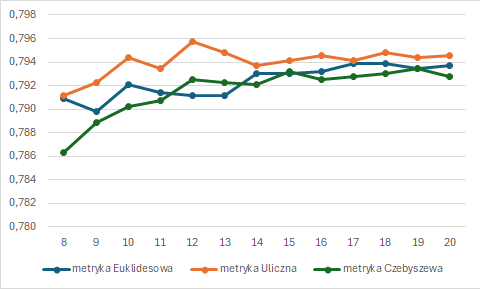
\includegraphics[width=1.0\textwidth]{plot.png}}
    \caption{Wykres zależności dokładności do wartości k}
    \label{fig:szum_jednostkowy_bin}
\end{figure}

\noindent Przyglądając się wynikom eksperymentu możemy zauważyć, że uzyskane wyniki są bez wątpienia zależne od wartości k. Dodatkowo uzyskane wyniki rosną wraz z wartością parametru, ale tylko do pewnego momentu, po uzyskaniu maksymalnej wartości dokładności wartość tej miary spada i mimo niewielkich wahań nigdy nie uzyskuje wyników wyższych niż wspomniana wcześniej wartość. \\

\noindent Mimo że uzyskane wartości miar jakości są bardzo podobne dla każdej z metryk to najwyższą dokładność uzyskaliśmy dla metryki Ulicznej przy k wynoszącym 12. \\

\newpage

\noindent Kolejnym faktem, który należy wypunktować jest powtarzająca się przewaga wartości czułości nad miarą precyzji. Jeśli precision jest niższa niż recall, to model częściej popełnia błędy typu fałszywie pozytywne niż fałszywie negatywne. Innymi słowy, jest bardziej skłonny do błędnie identyfikowania wyników jako pozytywne, nawet gdy są one fałszywe. Może to oznaczać, że model jest zbyt optymistyczny w klasyfikowaniu przypadków. \\

\noindent Należy również zauważyć, że istnieje wiele wartości wynoszących 0 bądź też wartości do 0 zbliżone, może to być spowodowane tym, że niektóre kraje są znacznie mniej licznie reprezentowane niż inne. W przypadku tych słabo reprezentowanych klas, model może mieć trudności w wyuczeniu się cech charakterystycznych dla tych klas, co prowadzi do niskich wartości miar jakości klasyfikacji.

\subsubsection*{Badanie wpływu rozkładu danych}

Przez rozkład danych biorących udział w badaniu rozumiemy jaką część danych, które mamy do dyspozycji bierzemy jako dane testowe a jakie dane uczące. Eksperymentowi poddane zostaną wszystkie metryki. Nadal operować będziemy na wcześniej przygotowanym zestawie danych. Podczas poprzednich badań przyjęty podział wyglądał następująco: 30\% danych testowych do 70\% danych uczących. Teraz pod rozważania poddane zostaną inne rozkłady między zbiorami danych, pozostałe wartości pozostają bez zmian i wyglądają następująco: \\

\noindent Dla metryki Euklidesowej wartość k wynosi 17, dla metryki Ulicznej k = 12 a dla metryki Czebyszewa przyjęte zostało k równe 19. Są to wartości, dla których w poprzednim eksperymencie uzyskane wyniki były najwyższe, pozwoli to na dalsze pogłębianie poszukiwań najlepszych kombinacji parametrów.\\

\noindent Z racji na fakt, że przyjęty zbiór danych nie pozwala na podział równy, wartości zostaną zaokrąglone w dół w kierunku zbioru testowego. Poniższe tabele zawierają wyniki eksperymentu dla każdej z metryk z uwzględnieniem wartości jednostkowych dla każdego z badanych krajów:

\newpage
\thispagestyle{empty}
\begin{table}[H]
    \centering
    \caption{Wpływ udziału danych uczących do danych testowych na wyniki klasyfikacji dla metryki Euklidesowej\\}
    \label{tab:my_label765}
    \begin{tabular}{|c|c|c|c|c|c|} 
        \hline 
        \multirow{2}{*}{\begin{tabular}{@{}c@{}} \% udział \\ danych testowych \end{tabular}} & \multirow{2}{*}{Wartości ogólne} & \multicolumn{4}{|c|}{Wartości jednostkowe} \\ 
        \cline{3-6}
         & & kraj & precyzja & czułość & f1 \\ 
        \hline

        10 \% &  
        \begin{tabular}{@{}c@{}}
        accuracy: 0.8117 \\
        precisionC: 0.8134 \\
        recallC: 0.9959 \\
        f1C: 0.8955
        \end{tabular} & 
        \begin{tabular}{@{}c@{}}
        usa: \\ 
        canada: \\
        japan: \\
        uk: \\  
        france: \\
        west-germany \\
        \end{tabular} &
        \begin{tabular}{@{}c@{}}
        \\
        0.8130 \\ 
        0.0000 \\
        0.0000 \\
        1.0000 \\  
        0.0000 \\
        0.0000 \\
        \\
        \end{tabular} &   
        \begin{tabular}{@{}c@{}}
        \\
        0.9983 \\ 
        0.0000 \\
        0.0000 \\
        0.0357 \\  
        0.0000 \\
        0.0000 \\
        \\
        \end{tabular} & 
        \begin{tabular}{@{}c@{}}
        \\
        0.8962 \\ 
        0.0000 \\
        0.0000 \\
        0.0690 \\  
        0.0000 \\
        0.0000 \\
        \\
        \end{tabular} \\
        \hline

        20 \% &  
        \begin{tabular}{@{}c@{}}
        accuracy: 0.8032 \\
        precisionC: 0.8050 \\
        recallC: 0.9966 \\
        f1C: 0.8907
        \end{tabular} & 
        \begin{tabular}{@{}c@{}}
        usa: \\ 
        canada: \\
        japan: \\
        uk: \\  
        france: \\
        west-germany \\
        \end{tabular} &
        \begin{tabular}{@{}c@{}}
        \\
        0.8055 \\ 
        0.0000 \\
        0.1250 \\
        0.7143 \\  
        0.0000 \\
        0.0000 \\
        \\
        \end{tabular} &   
        \begin{tabular}{@{}c@{}}
        \\
        0.9991 \\ 
        0.0000 \\
        0.0149 \\
        0.0249 \\  
        0.0000 \\
        0.0000 \\
        \\
        \end{tabular} & 
        \begin{tabular}{@{}c@{}}
        \\
        0.8920 \\ 
        0.0000 \\
        0.0267 \\
        0.0481 \\  
        0.0000 \\
        0.0000 \\
        \\
        \end{tabular} \\
        \hline

        30 \% &  
        \begin{tabular}{@{}c@{}}
        accuracy: 0.7939 \\
        precisionC: 0.7952 \\
        recallC: 0.9958 \\
        f1C: 0.8843
        \end{tabular} & 
        \begin{tabular}{@{}c@{}}
        usa: \\ 
        canada: \\
        japan: \\
        uk: \\  
        france: \\
        west-germany \\
        \end{tabular} &
        \begin{tabular}{@{}c@{}}
        \\
        0.7964 \\ 
        0.0000 \\
        0.3333 \\
        0.5455 \\  
        0.0000 \\
        0.0000 \\
        \\
        \end{tabular} &   
        \begin{tabular}{@{}c@{}}
        \\
        0.9991 \\ 
        0.0000 \\
        0.0444 \\
        0.0193 \\  
        0.0000 \\
        0.0000 \\
        \\
        \end{tabular} & 
        \begin{tabular}{@{}c@{}}
        \\
        0.8864 \\ 
        0.0000 \\
        0.0784 \\
        0.0373 \\  
        0.0000 \\
        0.0000 \\
        \\
        \end{tabular} \\
        \hline

        40 \% &  
        \begin{tabular}{@{}c@{}}
        accuracy: 0.7939 \\
        precisionC: 0.7954 \\
        recallC: 0.9962 \\
        f1C: 0.8846
        \end{tabular} & 
        \begin{tabular}{@{}c@{}}
        usa: \\ 
        canada: \\
        japan: \\
        uk: \\  
        france: \\
        west-germany \\
        \end{tabular} &
        \begin{tabular}{@{}c@{}}
        \\
        0.7964 \\ 
        0.0000 \\
        0.2857 \\
        0.5000 \\  
        0.0000 \\
        0.0000 \\
        \\
        \end{tabular} &   
        \begin{tabular}{@{}c@{}}
        \\
        0.9985 \\ 
        0.0000 \\
        0.0370 \\
        0.0119 \\  
        0.0000 \\
        0.0000 \\
        \\
        \end{tabular} & 
        \begin{tabular}{@{}c@{}}
        \\
        0.8861 \\ 
        0.0000 \\
        0.0656 \\
        0.0232 \\  
        0.0000 \\
        0.0000 \\
        \\
        \end{tabular} \\
        \hline

        50 \% &  
        \begin{tabular}{@{}c@{}}
        accuracy: 0.7919 \\
        precisionC: 0.7936 \\
        recallC: 0.9962 \\
        f1C: 0.8834
        \end{tabular} & 
        \begin{tabular}{@{}c@{}}
        usa: \\ 
        canada: \\
        japan: \\
        uk: \\  
        france: \\
        west-germany \\
        \end{tabular} &
        \begin{tabular}{@{}c@{}}
        \\
        0.7944 \\ 
        1.0000 \\
        0.2000 \\
        0.5556 \\  
        0.0000 \\
        0.3333 \\
        \\
        \end{tabular} &   
        \begin{tabular}{@{}c@{}}
        \\
        0.9983 \\ 
        0.0021 \\
        0.0238 \\
        0.0090 \\  
        0.0000 \\
        0.0062 \\
        \\
        \end{tabular} & 
        \begin{tabular}{@{}c@{}}
        \\
        0.8847 \\ 
        0.0042 \\
        0.0426 \\
        0.0178 \\  
        0.0000 \\
        0.0121 \\
        \\
        \end{tabular} \\
        \hline

        60 \% &  
        \begin{tabular}{@{}c@{}}
        accuracy: 0.7892 \\
        precisionC: 0.7900 \\
        recallC: 0.9970 \\
        f1C: 0.8815
        \end{tabular} & 
        \begin{tabular}{@{}c@{}}
        usa: \\ 
        canada: \\
        japan: \\
        uk: \\  
        france: \\
        west-germany \\
        \end{tabular} &
        \begin{tabular}{@{}c@{}}
        \\
        0.7907 \\ 
        0.0000 \\
        0.3889 \\
        0.4000 \\  
        0.0000 \\
        0.5000 \\
        \\
        \end{tabular} &   
        \begin{tabular}{@{}c@{}}
        \\
        0.9987 \\ 
        0.0000 \\
        0.0233 \\
        0.0060 \\  
        0.0000 \\
        0.0048 \\
        \\
        \end{tabular} & 
        \begin{tabular}{@{}c@{}}
        \\
        0.8826 \\ 
        0.0000 \\
        0.0440 \\
        0.0119 \\  
        0.0000 \\
        0.0094 \\
        \\
        \end{tabular} \\
        \hline    

    \end{tabular}  
\end{table}

\thispagestyle{empty}
\begin{table}[H]
    \centering
    \caption{Wpływ udziału danych uczących do danych testowych na wyniki klasyfikacji dla metryki Ulicznej\\}
    \label{tab:my_label4231}
    \begin{tabular}{|c|c|c|c|c|c|} 
        \hline 
        \multirow{2}{*}{\begin{tabular}{@{}c@{}} \% udział \\ danych testowych \end{tabular}} & \multirow{2}{*}{Wartości ogólne} & \multicolumn{4}{|c|}{Wartości jednostkowe} \\ 
        \cline{3-6}
         & & kraj & precyzja & czułość & f1 \\ 
        \hline

        10 \% &  
        \begin{tabular}{@{}c@{}}
        accuracy: 0.8117 \\
        precisionC: 0.8148 \\
        recallC: 0.9893 \\
        f1C: 0.8936
        \end{tabular} & 
        \begin{tabular}{@{}c@{}}
        usa: \\ 
        canada: \\
        japan: \\
        uk: \\  
        france: \\
        west-germany \\
        \end{tabular} &
        \begin{tabular}{@{}c@{}}
        \\
        0.8158 \\ 
        1.0000 \\
        0.0000 \\
        0.5000 \\  
        0.0000 \\
        0.0000 \\
        \\
        \end{tabular} &   
        \begin{tabular}{@{}c@{}}
        \\
        0.9949 \\ 
        0.0174 \\
        0.0000 \\
        0.0595 \\  
        0.0000 \\
        0.0000 \\
        \\
        \end{tabular} & 
        \begin{tabular}{@{}c@{}}
        \\
        0.8965 \\ 
        0.0342 \\
        0.0000 \\
        0.1064 \\  
        0.0000 \\
        0.0000 \\
        \\
        \end{tabular} \\
        \hline

        20 \% &  
        \begin{tabular}{@{}c@{}}
        accuracy: 0.8021 \\
        precisionC: 0.8058 \\
        recallC: 0.9920 \\
        f1C: 0.8892 
        \end{tabular} & 
        \begin{tabular}{@{}c@{}}
        usa: \\ 
        canada: \\
        japan: \\
        uk: \\  
        france: \\
        west-germany \\
        \end{tabular} &
        \begin{tabular}{@{}c@{}}
        \\
        0.8073 \\ 
        0.6667 \\
        0.0909 \\
        0.4375 \\  
        0.0000 \\
        0.0000 \\
        \\
        \end{tabular} &   
        \begin{tabular}{@{}c@{}}
        \\
        0.9961 \\ 
        0.0090 \\
        0.0149 \\
        0.0348 \\  
        0.0000 \\
        0.0000 \\
        \\
        \end{tabular} & 
        \begin{tabular}{@{}c@{}}
        \\
        0.8918 \\ 
        0.0178 \\
        0.0256 \\
        0.0645 \\  
        0.0000 \\
        0.0000 \\
        \\
        \end{tabular} \\
        \hline

        30 \% &  
        \begin{tabular}{@{}c@{}}
        accuracy: 0.7957 \\
        precisionC: 0.7977 \\
        recallC: 0.9930 \\
        f1C: 0.8847
        \end{tabular} & 
        \begin{tabular}{@{}c@{}}
        usa: \\ 
        canada: \\
        japan: \\
        uk: \\  
        france: \\
        west-germany \\
        \end{tabular} &
        \begin{tabular}{@{}c@{}}
        \\
        0.7997 \\ 
        0.7500 \\
        0.3333 \\
        0.5000 \\  
        0.0000 \\
        0.0000 \\
        \\
        \end{tabular} &   
        \begin{tabular}{@{}c@{}}
        \\
        0.9988 \\ 
        0.0096 \\
        0.0593 \\
        0.0322 \\  
        0.0000 \\
        0.0000 \\
        \\
        \end{tabular} & 
        \begin{tabular}{@{}c@{}}
        \\
        0.8883 \\ 
        0.0189 \\
        0.1006 \\
        0.0604 \\  
        0.0000 \\
        0.0000 \\
        \\
        \end{tabular} \\
        \hline

        40 \% &  
        \begin{tabular}{@{}c@{}}
        accuracy: 0.7953 \\
        precisionC: 0.7979 \\
        recallC: 0.9945 \\
        f1C: 0.8855
        \end{tabular} & 
        \begin{tabular}{@{}c@{}}
        usa: \\ 
        canada: \\
        japan: \\
        uk: \\  
        france: \\
        west-germany \\
        \end{tabular} &
        \begin{tabular}{@{}c@{}}
        \\
        0.7997 \\ 
        0.5000 \\
        0.3000 \\
        0.4091 \\  
        0.0000 \\
        0.0000 \\
        \\
        \end{tabular} &   
        \begin{tabular}{@{}c@{}}
        \\
        0.9985 \\ 
        0.0024 \\
        0.0559 \\
        0.0214 \\  
        0.0000 \\
        0.0000 \\
        \\
        \end{tabular} & 
        \begin{tabular}{@{}c@{}}
        \\
        0.8881 \\ 
        0.0049 \\
        0.0942 \\
        0.0406 \\  
        0.0000 \\
        0.0000 \\
        \\
        \end{tabular} \\
        \hline

        50 \% &  
        \begin{tabular}{@{}c@{}}
        accuracy: 0.7923 \\
        precisionC: 0.7954 \\
        recallC: 0.9927 \\
        f1C: 0.8832
        \end{tabular} & 
        \begin{tabular}{@{}c@{}}
        usa: \\ 
        canada: \\
        japan: \\
        uk: \\  
        france: \\
        west-germany \\
        \end{tabular} &
        \begin{tabular}{@{}c@{}}
        \\
        0.7973 \\ 
        0.8000 \\
        0.2558 \\
        0.3636 \\  
        0.0000 \\
        0.3750 \\
        \\
        \end{tabular} &   
        \begin{tabular}{@{}c@{}}
        \\
        0.9970 \\ 
        0.0083 \\
        0.0521 \\
        0.0145 \\  
        0.0000 \\
        0.0185 \\
        \\
        \end{tabular} & 
        \begin{tabular}{@{}c@{}}
        \\
        0.8860 \\ 
        0.0165 \\
        0.0866 \\
        0.0279 \\  
        0.0000 \\
        0.0353 \\
        \\
        \end{tabular} \\
        \hline

        60 \% &  
        \begin{tabular}{@{}c@{}}
        accuracy: 0.7886 \\
        precisionC: 0.7912 \\
        recallC: 0.9913 \\
        f1C: 0.8800
        \end{tabular} & 
        \begin{tabular}{@{}c@{}}
        usa: \\ 
        canada: \\
        japan: \\
        uk: \\  
        france: \\
        west-germany \\
        \end{tabular} &
        \begin{tabular}{@{}c@{}}
        \\
        0.7931 \\ 
        0.4444 \\
        0.3171 \\
        0.4000 \\  
        0.0000 \\
        0.0000 \\
        \\
        \end{tabular} &   
        \begin{tabular}{@{}c@{}}
        \\
        0.9956 \\ 
        0.0073 \\
        0.0432 \\
        0.0211 \\  
        0.0000 \\
        0.0000 \\
        \\
        \end{tabular} & 
        \begin{tabular}{@{}c@{}}
        \\
        0.8829 \\ 
        0.0143 \\
        0.0760 \\
        0.0400 \\  
        0.0000 \\
        0.0000 \\
        \\
        \end{tabular} \\
        \hline    

    \end{tabular}  
\end{table}

\thispagestyle{empty}
\begin{table}[H]
    \centering
    \caption{Wpływ udziału danych uczących do danych testowych na wyniki klasyfikacji dla metryki Czebyszewa \\}
    \label{tab:my_label35345}
    \begin{tabular}{|c|c|c|c|c|c|} 
        \hline 
        \multirow{2}{*}{\begin{tabular}{@{}c@{}} \% udział \\ danych testowych \end{tabular}} & \multirow{2}{*}{Wartości ogólne} & \multicolumn{4}{|c|}{Wartości jednostkowe} \\ 
        \cline{3-6}
         & & kraj & precyzja & czułość & f1 \\ 
        \hline

        10 \% &  
        \begin{tabular}{@{}c@{}}
        accuracy: 0.8103 \\
        precisionC: 0.8122 \\
        recallC: 0.9925 \\
        f1C: 0.8933 \\
        \end{tabular} & 
        \begin{tabular}{@{}c@{}}
        usa: \\ 
        canada: \\
        japan: \\
        uk: \\  
        france: \\
        west-germany \\
        \end{tabular} &
        \begin{tabular}{@{}c@{}}
        \\
        0.8131 \\ 
        1.0000 \\
        0.0000 \\
        0.3750 \\  
        0.0000 \\
        0.0000 \\
        \\
        \end{tabular} &   
        \begin{tabular}{@{}c@{}}
        \\
        0.9958 \\ 
        0.0087 \\
        0.0000 \\
        0.0357 \\  
        0.0000 \\
        0.0000 \\
        \\
        \end{tabular} & 
        \begin{tabular}{@{}c@{}}
        \\
        0.8952 \\ 
        0.0172 \\
        0.0000 \\
        0.0652 \\  
        0.0000 \\
        0.0000 \\
        \\
        \end{tabular} \\
        \hline

        20 \% &  
        \begin{tabular}{@{}c@{}}
        accuracy: 0.8018 \\
        precisionC: 0.8040 \\
        recallC: 0.9949 \\
        f1C: 0.8893
        \end{tabular} & 
        \begin{tabular}{@{}c@{}}
        usa: \\ 
        canada: \\
        japan: \\
        uk: \\  
        france: \\
        west-germany \\
        \end{tabular} &
        \begin{tabular}{@{}c@{}}
        \\
        0.8050 \\ 
        0.6667 \\
        0.1250 \\
        0.3750 \\  
        0.0000 \\
        0.0000 \\
        \\
        \end{tabular} &   
        \begin{tabular}{@{}c@{}}
        \\
        0.9974 \\ 
        0.0090 \\
        0.0149 \\
        0.0149 \\  
        0.0000 \\
        0.0000 \\
        \\
        \end{tabular} & 
        \begin{tabular}{@{}c@{}}
        \\
        0.8909 \\ 
        0.0178 \\
        0.0267 \\
        0.0287 \\  
        0.0000 \\
        0.0000 \\
        \\
        \end{tabular} \\
        \hline

        30 \% &  
        \begin{tabular}{@{}c@{}}
        accuracy: 0.7935 \\
        precisionC: 0.7947 \\
        recallC: 0.9955 \\
        f1C: 0.8838
        \end{tabular} & 
        \begin{tabular}{@{}c@{}}
        usa: \\ 
        canada: \\
        japan: \\
        uk: \\  
        france: \\
        west-germany \\
        \end{tabular} &
        \begin{tabular}{@{}c@{}}
        \\
        0.7960 \\ 
        0.0000 \\
        0.4000 \\
        0.4444 \\  
        0.0000 \\
        0.0000 \\
        \\
        \end{tabular} &   
        \begin{tabular}{@{}c@{}}
        \\
        0.9988 \\ 
        0.0000 \\
        0.0588 \\
        0.0129 \\  
        0.0000 \\
        0.0000 \\
        \\
        \end{tabular} & 
        \begin{tabular}{@{}c@{}}
        \\
        0.8860 \\ 
        0.0000 \\
        0.1026 \\
        0.0251 \\  
        0.0000 \\
        0.0000 \\
        \\
        \end{tabular} \\
        \hline

        40 \% &  
        \begin{tabular}{@{}c@{}}
        accuracy: 0.7937 \\
        precisionC: 0.7953 \\
        recallC: 0.9964 \\
        f1C: 0.8845
        \end{tabular} & 
        \begin{tabular}{@{}c@{}}
        usa: \\ 
        canada: \\
        japan: \\
        uk: \\  
        france: \\
        west-germany \\
        \end{tabular} &
        \begin{tabular}{@{}c@{}}
        \\
        0.7963 \\ 
        0.0000 \\
        0.3000 \\
        0.3636 \\  
        0.0000 \\
        0.0000 \\
        \\
        \end{tabular} &   
        \begin{tabular}{@{}c@{}}
        \\
        0.9985 \\ 
        0.0000 \\
        0.0370 \\
        0.0095 \\  
        0.0000 \\
        0.0000 \\
        \\
        \end{tabular} & 
        \begin{tabular}{@{}c@{}}
        \\
        0.8860 \\ 
        0.0000 \\
        0.0659 \\
        0.0185 \\  
        0.0000 \\
        0.0000 \\
        \\
        \end{tabular} \\
        \hline

        50 \% &  
        \begin{tabular}{@{}c@{}}
        accuracy: 0.7913 \\
        precisionC: 0.7934 \\
        recallC: 0.9976 \\
        f1C: 0.8838
        \end{tabular} & 
        \begin{tabular}{@{}c@{}}
        usa: \\ 
        canada: \\
        japan: \\
        uk: \\  
        france: \\
        west-germany \\
        \end{tabular} &
        \begin{tabular}{@{}c@{}}
        \\
        0.7940 \\ 
        0.0000 \\
        0.1852 \\
        0.2000 \\  
        0.0000 \\
        0.0000 \\
        \\
        \end{tabular} &   
        \begin{tabular}{@{}c@{}}
        \\
        0.9986 \\ 
        0.0000 \\
        0.0238 \\
        0.0018 \\  
        0.0000 \\
        0.0000 \\
        \\
        \end{tabular} & 
        \begin{tabular}{@{}c@{}}
        \\
        0.8846 \\ 
        0.0000 \\
        0.0422 \\
        0.0036 \\  
        0.0000 \\
        0.0000 \\
        \\
        \end{tabular} \\
        \hline

        60 \% &  
        \begin{tabular}{@{}c@{}}
        accuracy: 0.7880 \\
        precisionC: 0.7900 \\
        recallC: 0.9968 \\
        f1C: 0.8814
        \end{tabular} & 
        \begin{tabular}{@{}c@{}}
        usa: \\ 
        canada: \\
        japan: \\
        uk: \\  
        france: \\
        west-germany \\
        \end{tabular} &
        \begin{tabular}{@{}c@{}}
        \\
        0.7904 \\ 
        0.0000 \\
        0.3333 \\
        0.0000 \\  
        0.0000 \\
        0.0000 \\
        \\
        \end{tabular} &   
        \begin{tabular}{@{}c@{}}
        \\
        0.9978 \\ 
        0.0000 \\
        0.0233 \\
        0.0000 \\  
        0.0000 \\
        0.0000 \\
        \\
        \end{tabular} & 
        \begin{tabular}{@{}c@{}}
        \\
        0.8821 \\ 
        0.0000 \\
        0.0435 \\
        0.0000 \\  
        0.0000 \\
        0.0000 \\
        \\
        \end{tabular} \\
        \hline    

    \end{tabular}  
\end{table}

\thispagestyle{empty}
\newpage

\subsubsection*{Podsumowanie eksperymentu}

\noindent Przeprowadzony eksperyment wykazał, że najlepsze wyniki klasyfikacji uzyskano dla proporcji 10\% danych testowych do 90\% danych uczących. W tym przypadku uzyskaliśmy precyzję na poziomie 81.17\% dla metryki Euklidesowej, dla metryki Ulicznej wartość tej miary jest tożsama dla metryki Czebyszewa wartość ta wynosi natomiast 81.03\% . Wyniki te sugerują, że w kontekście analizowanego zbioru danych ta proporcja podziału danych jest optymalna, pozwalając na osiągnięcie najlepszej jakości klasyfikacji. \\

\noindent Warto tutaj zaznaczyć, że mimo osiągnięcia tej samej dokładności metryka Euklidesa posiada nieco wyższą wartość miary F1, różnica tych wartości \\ (0,895459629984927 dla metryki Euklidesa oraz 0,893622118 dla metryki Ulicznej) wynosi dokładnie 0,001837512 tak więc w przypadku naszego klasyfikatora metryka Euklidesa zwraca najlepsze wyniki. \\

\noindent Dodatkowo możemy zauważyć, że wyższy procentowy udział danych testowych do uczących powoduje znaczący spadek w jakości klasyfikacji, jedynym odstępstwem od tej normy jest metryka uliczna, która nawet dla 60\% udziału danych testowych radzi sobie lepiej od pozostałych metryk. \\


\subsubsection*{Badanie wpływu konkretnych cech}

\noindent W celu zbadania tego, jak konkretne cechy wpływają na otrzymywany wynik, utworzono 4 grupy cech, dla których wszystkie pozostałe zmienne pozostają takie same. Wykonane zostaną kolejno badania dla każdej z badanych metryk. Dla każdej z nich udział danych testowych do danych uczących wynosi 10\%. Dodatkowo dla każdej z nich zastosowana została wartość k, zwracająca najlepsze wartości. Czyli dla metryki Euklidesowej wartość ta wynosi 17, dla metryki Ulicznej 12, a dla metryki Czebyszewa 19." \\

\noindent \textbf{I grupa: } pierwszą z utworzonych grup stanowi zbiór cech z wyłączeniem cech słownikowych, czyli nawiązując do drugiej sekcji dokumentu będą to cechy bez cech 1-3. \\

\noindent \textbf{II grupa: } kolejną grupę stanowić będą wszystkie cechy poza cechami 4, 5 oraz 6 (ponownie nawiązując do drugiej sekcji sprawozdania). Wyłączone cechy mówią o ilości słów spełniających zadane kryteria. \\

\noindent \textbf{III grupa: } trzecią grupę stanowić będą cechy 1-6 oraz 9 i 10, cechy wyłączone (7,8) mówią o długościach słów. \\

\noindent \textbf{IV grupa: } ostatnia grupa złożona jest z cech z wyłączeniem cech 9 oraz 10. W skład ten wchodzi więc cechy zliczająca ilość znaków w najdłuższym słowie oraz cecha zliczająca wystąpienia słów zawierających. "\textendash".

\noindent warto wspomnieć, że podczas badania wpływu poszczególnych cech należy je wyłączyć z eksperymentu. Jest to spowodowane faktem, że klasyfikator, działając na małej liczbie cech, może napotkać znaczne trudności w odpowiednim opisaniu tekstów. \\

\noindent Stosując metodę wyłączenia badanych cech, będziemy mogli ocenić, czy klasyfikator, działający bez wspomnianych cech, zwraca gorsze wyniki. W takim przypadku można wnioskować, że te cechy mają pozytywny wpływ na wyniki klasyfikacji. Jeśli otrzymane wyniki pozostają niezmienione, można zakładać, że badane cechy nie mają wpływu na wyniki algorytmu. Natomiast, jeśli otrzymane wyniki są wyższe niż te uzyskane przy pracy klasyfikatora na wszystkich cechach, można przyjąć, że badane cechy szkodzą klasyfikatorowi. \\


\begin{table}[H]
    \centering
    \caption{Wpływ poszczegółnych zbiorów cech na wyniki klasyfikatora dla metryki Euklidesa \\}
    \label{tab:my_label_jkhbnik}
    \begin{tabular}{|c|c|c|c|c|c|} 
        \hline 
        \multirow{2}{*}{Zewstaw cech} & \multirow{2}{*}{Wartości ogólne} & \multicolumn{4}{|c|}{Wartości jednostkowe} \\ 
        \cline{3-6}
         & & kraj & precyzja & czułość & f1 \\ 
        \hline

        I &  
        \begin{tabular}{@{}c@{}}
        accuracy: 0.8117 \\
        precisionC: 0.8134 \\
        recallC: 0.9959 \\
        f1C: 0.8955
        \end{tabular} & 
        \begin{tabular}{@{}c@{}}
        usa: \\ 
        canada: \\
        japan: \\
        uk: \\  
        france: \\
        west-germany \\
        \end{tabular} &
        \begin{tabular}{@{}c@{}}
        \\
        0.8130 \\ 
        0.0000 \\
        0.0000 \\
        1.0000 \\  
        0.0000 \\
        0.0000 \\
        \\
        \end{tabular} &   
        \begin{tabular}{@{}c@{}}
        \\
        0.9983 \\ 
        0.0000 \\
        0.0000 \\
        0.0357 \\  
        0.0000 \\
        0.0000 \\
        \\
        \end{tabular} & 
        \begin{tabular}{@{}c@{}}
        \\
        0.8962 \\ 
        0.0000 \\
        0.0000 \\
        0.0690 \\  
        0.0000 \\
        0.0000 \\
        \\
        \end{tabular} \\
        \hline

%===================================================================

        II &  
        \begin{tabular}{@{}c@{}}
        accuracy: 0.8131 \\
        precisionC: 0.8143 \\
        recallC: 0.9927 \\
        f1C: 0.8947
        \end{tabular} & 
        \begin{tabular}{@{}c@{}}
        usa: \\ 
        canada: \\
        japan: \\
        uk: \\  
        france: \\
        west-germany \\
        \end{tabular} &
        \begin{tabular}{@{}c@{}}
        \\
        0.8157 \\ 
        0.5000 \\
        0.0000 \\
        0.5556 \\  
        0.0000 \\
        0.0000 \\
        \\
        \end{tabular} &   
        \begin{tabular}{@{}c@{}}
        \\
        0.9975 \\ 
        0.0088 \\
        0.0000 \\
        0.0595 \\  
        0.0000 \\
        0.0000 \\
        \\
        \end{tabular} & 
        \begin{tabular}{@{}c@{}}
        \\
        0.8974 \\ 
        0.0172 \\
        0.0000 \\
        0.1075 \\  
        0.0000 \\
        0.0000 \\
        \\
        \end{tabular} \\
        \hline

%===================================================================

        III &  
        \begin{tabular}{@{}c@{}}
        accuracy: 0.8131 \\
        precisionC: 0.8132 \\
        recallC: 0.9958 \\
        f1C: 0.8953
        \end{tabular} & 
        \begin{tabular}{@{}c@{}}
        usa: \\ 
        canada: \\
        japan: \\
        uk: \\  
        france: \\
        west-germany \\
        \end{tabular} &
        \begin{tabular}{@{}c@{}}
        \\
        0.8131 \\ 
        0.6667 \\
        0.0000 \\
        1.0000 \\  
        0.0000 \\
        0.0000 \\
        \\
        \end{tabular} &   
        \begin{tabular}{@{}c@{}}
        \\
        0.9992 \\ 
        0.0174 \\
        0.0000 \\
        0.0238 \\  
        0.0000 \\
        0.0000 \\
        \\
        \end{tabular} & 
        \begin{tabular}{@{}c@{}}
        \\
        0.8966 \\ 
        0.0339 \\
        0.0000 \\
        0.0465 \\  
        0.0000 \\
        0.0000 \\
        \\
        \end{tabular} \\
        \hline

%===================================================================

        IV &  
        \begin{tabular}{@{}c@{}}
        accuracy: 0.8082 \\
        precisionC: 0.8111 \\
        recallC: 0.9949 \\
        f1C: 0.8936 
        \end{tabular} & 
        \begin{tabular}{@{}c@{}}
        usa: \\ 
        canada: \\
        japan: \\
        uk: \\  
        france: \\
        west-germany \\
        \end{tabular} &
        \begin{tabular}{@{}c@{}}
        \\
        0.8115 \\ 
        0.3333 \\
        0.0000 \\
        0.0000 \\
        0.0000 \\
        0.0000 \\
        \\
        \end{tabular} &   
        \begin{tabular}{@{}c@{}}
        \\
        0.9958 \\ 
        0.0087 \\
        0.0000 \\
        0.0000 \\
        0.0000 \\
        0.0000 \\
        \\
        \end{tabular} & 
        \begin{tabular}{@{}c@{}}
        \\
        0.8942 \\ 
        0.0169 \\
        0.0000 \\
        0.0000 \\
        0.0000 \\
        0.0000 \\
        \\
        \end{tabular} \\
        \hline



    \end{tabular}  
\end{table}

        
\begin{table}[H]
    \centering
    \caption{Wpływ poszczególnych zbiorów cech na wyniki klasyfikatora dla metryki Ulicznej \\}
    \label{tab:my_label_jktiaik}
    \begin{tabular}{|c|c|c|c|c|c|} 
        \hline 
        \multirow{2}{*}{Zestaw cech} & \multirow{2}{*}{Wartości ogólne} & \multicolumn{4}{|c|}{Wartości jednostkowe} \\ 
        \cline{3-6}
         & & kraj & precyzja & czułość & f1 \\ 
        \hline

        I &  
        \begin{tabular}{@{}c@{}}
        accuracy: 0.8117 \\
        precisionC: 0.8148 \\
        recallC: 0.9893 \\
        f1C: 0.8936
        \end{tabular} & 
        \begin{tabular}{@{}c@{}}
        usa: \\ 
        canada: \\
        japan: \\
        uk: \\  
        france: \\
        west-germany \\
        \end{tabular} &
        \begin{tabular}{@{}c@{}}
        \\
        0.8158 \\ 
        1.0000 \\
        0.0000 \\
        0.5000 \\  
        0.0000 \\
        0.0000 \\
        \\
        \end{tabular} &   
        \begin{tabular}{@{}c@{}}
        \\
        0.9949 \\ 
        0.0174 \\
        0.0000 \\
        0.0595 \\  
        0.0000 \\
        0.0000 \\
        \\
        \end{tabular} & 
        \begin{tabular}{@{}c@{}}
        \\
        0.8965 \\ 
        0.0342 \\
        0.0000 \\
        0.1064 \\  
        0.0000 \\
        0.0000 \\
        \\
        \end{tabular} \\
        \hline

        II &  
        \begin{tabular}{@{}c@{}}
        accuracy: 0.8192 \\
        precisionC: 0.8205 \\
        recallC: 0.9864 \\
        f1C: 0.8958
        \end{tabular} & 
        \begin{tabular}{@{}c@{}}
        usa: \\ 
        canada: \\
        japan: \\
        uk: \\  
        france: \\
        west-germany \\
        \end{tabular} &
        \begin{tabular}{@{}c@{}}
        \\
        0.8208 \\ 
        1.0000 \\
        0.0000 \\
        0.7500 \\  
        0.0000 \\
        0.0000 \\
        \\
        \end{tabular} &   
        \begin{tabular}{@{}c@{}}
        \\
        0.9975 \\ 
        0.0263 \\
        0.0000 \\
        0.1429 \\  
        0.0000 \\
        0.0000 \\
        \\
        \end{tabular} & 
        \begin{tabular}{@{}c@{}}
        \\
        0.9005 \\ 
        0.0513 \\
        0.0000 \\
        0.2400 \\  
        0.0000 \\
        0.0000 \\
        \\
        \end{tabular} \\
        \hline

        III &  
        \begin{tabular}{@{}c@{}}
        accuracy: 0.8103 \\
        precisionC: 0.8123 \\
        recallC: 0.9925 \\
        f1C: 0.8934
        \end{tabular} & 
        \begin{tabular}{@{}c@{}}
        usa: \\ 
        canada: \\
        japan: \\
        uk: \\  
        france: \\
        west-germany \\
        \end{tabular} &
        \begin{tabular}{@{}c@{}}
        \\
        0.8131 \\ 
        0.6000 \\
        0.0000 \\
        0.5000 \\  
        0.0000 \\
        0.0000 \\
        \\
        \end{tabular} &   
        \begin{tabular}{@{}c@{}}
        \\
        0.9958 \\ 
        0.0261 \\
        0.0000 \\
        0.0119 \\  
        0.0000 \\
        0.0000 \\
        \\
        \end{tabular} & 
        \begin{tabular}{@{}c@{}}
        \\
        0.8952 \\ 
        0.0500 \\
        0.0000 \\
        0.0233 \\  
        0.0000 \\
        0.0000 \\
        \\
        \end{tabular} \\
        \hline

        IV &  
        \begin{tabular}{@{}c@{}}
        accuracy: 0.8124 \\
        precisionC: 0.8138 \\
        recallC: 0.9917 \\
        f1C: 0.8940
        \end{tabular} & 
        \begin{tabular}{@{}c@{}}
        usa: \\ 
        canada: \\
        japan: \\
        uk: \\  
        france: \\
        west-germany \\
        \end{tabular} &
        \begin{tabular}{@{}c@{}}
        \\
        0.8144 \\ 
        0.8000 \\
        0.0000 \\
        0.5000 \\  
        0.0000 \\
        0.0000 \\
        \\
        \end{tabular} &   
        \begin{tabular}{@{}c@{}}
        \\
        0.9966 \\ 
        0.0348 \\
        0.0000 \\
        0.0238 \\  
        0.0000 \\
        0.0000 \\
        \\
        \end{tabular} & 
        \begin{tabular}{@{}c@{}}
        \\
        0.8963 \\ 
        0.0667 \\
        0.0000 \\
        0.0455 \\  
        0.0000 \\
        0.0000 \\
        \\
        \end{tabular} \\
        \hline

    \end{tabular}  
\end{table}
\begin{table}[H]
    \centering
    \caption{Wpływ poszczegółnych zbiorów cech na wyniki klasyfikatora dla metryki Czebyszewa \\}
    \label{tab:my_label_qweqqbnik}
    \begin{tabular}{|c|c|c|c|c|c|} 
        \hline 
        \multirow{2}{*}{Zewstaw cech} & \multirow{2}{*}{Wartości ogólne} & \multicolumn{4}{|c|}{Wartości jednostkowe} \\ 
        \cline{3-6}
         & & kraj & precyzja & czułość & f1 \\ 
        \hline

        I &  
        \begin{tabular}{@{}c@{}}
        accuracy: 0.8103 \\
        precisionC: 0.8122 \\
        recallC: 0.9925 \\
        f1C: 0.8933
        \end{tabular} & 
        \begin{tabular}{@{}c@{}}
        usa: \\ 
        canada: \\
        japan: \\
        uk: \\  
        france: \\
        west-germany \\
        \end{tabular} &
        \begin{tabular}{@{}c@{}}
        \\
        0.8131 \\ 
        1.0000 \\
        0.0000 \\
        0.3750 \\  
        0.0000 \\
        0.0000 \\
        \\
        \end{tabular} &   
        \begin{tabular}{@{}c@{}}
        \\
        0.9958 \\ 
        0.0087 \\
        0.0000 \\
        0.0357 \\  
        0.0000 \\
        0.0000 \\
        \\
        \end{tabular} & 
        \begin{tabular}{@{}c@{}}
        \\
        0.8952 \\ 
        0.0172 \\
        0.0000 \\
        0.0652 \\  
        0.0000 \\
        0.0000 \\
        \\
        \end{tabular} \\
        \hline

        II &  
        \begin{tabular}{@{}c@{}}
        accuracy: 0.8103 \\
        precisionC: 0.8114 \\
        recallC: 0.999 \\
        f1C: 0.8956
        \end{tabular} & 
        \begin{tabular}{@{}c@{}}
        usa: \\ 
        canada: \\
        japan: \\
        uk: \\  
        france: \\
        west-germany \\
        \end{tabular} &
        \begin{tabular}{@{}c@{}}
        \\
        0.8114 \\ 
        0.0000 \\
        0.0000 \\
        0.0000 \\  
        0.0000 \\
        0.0000 \\
        \\
        \end{tabular} &   
        \begin{tabular}{@{}c@{}}
        \\
        0.9992 \\ 
        0.0000 \\
        0.0000 \\
        0.0000 \\  
        0.0000 \\
        0.0000 \\
        \\
        \end{tabular} & 
        \begin{tabular}{@{}c@{}}
        \\
        0.8956 \\ 
        0.0000 \\
        0.0000 \\
        0.0000 \\  
        0.0000 \\
        0.0000 \\
        \\
        \end{tabular} \\
        \hline

        III &  
        \begin{tabular}{@{}c@{}}
        accuracy: 0.8131 \\
        precisionC: 0.8131 \\
        recallC: 0.9975 \\
        f1C: 0.8960
        \end{tabular} & 
        \begin{tabular}{@{}c@{}}
        usa: \\ 
        canada: \\
        japan: \\
        uk: \\  
        france: \\
        west-germany \\
        \end{tabular} &
        \begin{tabular}{@{}c@{}}
        \\
        0.8127 \\ 
        1.0000 \\
        0.0000 \\
        0.0000 \\  
        0.0000 \\
        0.0000 \\
        \\
        \end{tabular} &   
        \begin{tabular}{@{}c@{}}
        \\
        1.0000 \\ 
        0.0261\\
        0.0000 \\
        0.0000 \\  
        0.0000 \\
        0.0000 \\
        \\
        \end{tabular} & 
        \begin{tabular}{@{}c@{}}
        \\
        0.8967 \\ 
        0.0508 \\
        0.0000 \\
        0.0000 \\  
        0.0000 \\
        0.0000 \\
        \\
        \end{tabular} \\
        \hline

        IV &  
        \begin{tabular}{@{}c@{}}
        accuracy: 0.8096 \\
        precisionC: 0.8115 \\
        recallC: 0.9966 \\
        f1C: 0.8946
        \end{tabular} & 
        \begin{tabular}{@{}c@{}}
        usa: \\ 
        canada: \\
        japan: \\
        uk: \\  
        france: \\
        west-germany \\
        \end{tabular} &
        \begin{tabular}{@{}c@{}}
        \\
        0.8117 \\ 
        0.5000 \\
        0.0000 \\
        0.0000 \\  
        0.0000 \\
        0.0000 \\
        \\
        \end{tabular} &   
        \begin{tabular}{@{}c@{}}
        \\
        0.9975 \\ 
        0.0087 \\
        0.0000 \\
        0.0000 \\  
        0.0000 \\
        0.0000 \\
        \\
        \end{tabular} & 
        \begin{tabular}{@{}c@{}}
        \\
        0.8951 \\ 
        0.0171 \\
        0.0000 \\
        0.0000 \\  
        0.0000 \\
        0.0000 \\
        \\
        \end{tabular} \\
        \hline


    \end{tabular}  
\end{table}


\newpage

\subsubsection*{Podsumowanie eksperymentu}

W poniższej tabeli znajdują się wyniki dokładności dla każdej z grup, wraz z różnicą między najlepszym otrzymanym wynikiem dla każdej z metryk uzyskanym w poprzednim eksperymencie. Wyniki zostały zapisane z dużą dokładnością po przecinku ze względu na to, że różnice między nimi są bardzo niewielkie. \\

\begin{table}[H]
    \centering
    \caption{Wyniki dokładności dla różnych grup cech}
    \label{tab:wyniki}
    \begin{tabular}{|c|c|c|c|} \hline 
        & Metryka Euklidesowa & Metryka Uliczna & Metryka Czebyszewa \\ \hline 
        \begin{tabular}{@{}c@{}}Wyniki dokładności \\ uzyskane w \\ poprzedniej subsekcji\end{tabular} & 0.811683849 & 0.811683849 & 0.810309278 \\ \hline 
        I & 0.810996564 & 0.810309278 & 0.810309278 \\ \hline 
        $\Delta$ I & 0.000687285 & 0.00137457 & 0 \\ \hline 
        II & 0.813058419 & 0.819243986 & 0.810309278 \\ \hline 
        $\Delta$ II & -0.00137457 & -0.007560137 & 0 \\ \hline 
        III & 0.813058419 & 0.810309278 & 0.813058419 \\ \hline 
        $\Delta$ III & -0.00137457 & 0.00137457 & -0.002749141 \\ \hline 
        IV & 0.808247423 & 0.812371134 & 0.809621993 \\ \hline 
        $\Delta$ IV & 0.003436426 & -0.000687285 & 0.000687285 \\ \hline
    \end{tabular}
\end{table}



\noindent Tak jak zostało już wspomniane, różnice między wynikami dla wszystkich cech oraz dla poszczególnych grup cech są nad wyraz niewielkie, istnieją jednak wpływy każdej z wyłączonych grup cech na ostateczny wynik klasyfikacji. \\

\noindent Analiza wyników wskazuje, że niektóre cechy mogą mieć zarówno pozytywny, jak i negatywny wpływ na dokładność klasyfikacji. Na przykład, dla metryki Euklidesowej, wyłączenie niektórych cech może prowadzić do poprawy dokładności klasyfikacji, podczas gdy dla metryki Ulicznej takie wyłączenie może prowadzić do pogorszenia wyników. \\

\noindent Należy również zwrócić uwagę na fakt, że metryka Czebyszewa wydaje się najmniej wrażliwa na zmiany w wykorzystywanych cechach. Dodatkowo minimalnie negatywny wpływ cech słownikowych (grupa I) może być spowodowany prawdopodobnie wykorzystaniem dolara jako waluty uniwersalnej w większości tekstów. Z tego powodu cecha 2 może przyjmować wartości na rzecz USA. \\

\noindent Warto również zauważyć, że różnice między wynikami dla poszczególnych grup cech są nadzwyczaj małe, co może świadczyć o subtelnych wpływach poszczególnych cech na proces klasyfikacji. \\



%==============================================================================================


\section{Dyskusja, wnioski, sprawozdanie końcowe}

Już na pierwszy rzut oka widzimy, że przygotowany program działa zasadniczo poprawnie, najwyższa osiągnięta dokładność wyniosła 81.17\% (wynik uzyskany dla Metryki Euklidesowej, k = 17 oraz 10\% udziale danych testowych do uczących). Poniżej raz jeszcze przedstawione zostały najwyższe wyniki uzyskane dla każdej z metryk z uwzględnieniem wartości jednostkowych dla każdego z badanych krajów. \\

\begin{table}[H]
    \centering
    \caption{Wpływ udziału danych uczących do danych testowych na wyniki klasyfikacji dla metryki Euklidesowej}
    \label{tab:my_label765}
    \begin{tabular}{|c|c|c|c|c|c|c|} 
        \hline 
        \multirow{2}{*}{k} & \multirow{2}{*}{\begin{tabular}{@{}c@{}} \% udział \\ danych testowych \end{tabular}} & \multirow{2}{*}{Wartości ogólne} & \multicolumn{4}{|c|}{Wartości jednostkowe} \\ 
        & \multicolumn{1}{|c|}{} & & kraj & precyzja & czułość & f1 \\ 
        \hline

        17 & 10 \% &  
        \begin{tabular}{@{}c@{}}
        accuracy: 0.8117 \\
        precisionC: 0.8134 \\
        recallC: 0.9959 \\
        f1C: 0.8955
        \end{tabular} & 
        \begin{tabular}{@{}c@{}}
        usa: \\ 
        canada: \\
        japan: \\
        uk: \\  
        france: \\
        west-germany \\
        \end{tabular} &
        \begin{tabular}{@{}c@{}}
        \\
        0.8130 \\ 
        0.0000 \\
        0.0000 \\
        1.0000 \\  
        0.0000 \\
        0.0000 \\
        \\
        \end{tabular} &   
        \begin{tabular}{@{}c@{}}
        \\
        0.9983 \\ 
        0.0000 \\
        0.0000 \\
        0.0357 \\  
        0.0000 \\
        0.0000 \\
        \\
        \end{tabular} & 
        \begin{tabular}{@{}c@{}}
        \\
        0.8962 \\ 
        0.0000 \\
        0.0000 \\
        0.0690 \\  
        0.0000 \\
        0.0000 \\
        \\
        \end{tabular} \\
        \hline

        12 & 10 \% &  
                \begin{tabular}{@{}c@{}}
        accuracy: 0.8117 \\
        precisionC: 0.8148 \\
        recallC: 0.9893 \\
        f1C: 0.8936
        \end{tabular} & 
        \begin{tabular}{@{}c@{}}
        usa: \\ 
        canada: \\
        japan: \\
        uk: \\  
        france: \\
        west-germany \\
        \end{tabular} &
        \begin{tabular}{@{}c@{}}
        \\
        0.8158 \\ 
        1.0000 \\
        0.0000 \\
        0.5000 \\  
        0.0000 \\
        0.0000 \\
        \\
        \end{tabular} &   
        \begin{tabular}{@{}c@{}}
        \\
        0.9949 \\ 
        0.0174 \\
        0.0000 \\
        0.0595 \\  
        0.0000 \\
        0.0000 \\
        \\
        \end{tabular} & 
        \begin{tabular}{@{}c@{}}
        \\
        0.8965 \\ 
        0.0342 \\
        0.0000 \\
        0.1064 \\  
        0.0000 \\
        0.0000 \\
        \\
        \end{tabular} \\
        \hline

        19 & 10 \% &  
        \begin{tabular}{@{}c@{}}
        accuracy: 0.8103 \\
        precisionC: 0.8122 \\
        recallC: 0.9925 \\
        f1C: 0.8933 \\
        \end{tabular} & 
        \begin{tabular}{@{}c@{}}
        usa: \\ 
        canada: \\
        japan: \\
        uk: \\  
        france: \\
        west-germany \\
        \end{tabular} &
        \begin{tabular}{@{}c@{}}
        \\
        0.8131 \\ 
        1.0000 \\
        0.0000 \\
        0.3750 \\  
        0.0000 \\
        0.0000 \\
        \\
        \end{tabular} &   
        \begin{tabular}{@{}c@{}}
        \\
        0.9958 \\ 
        0.0087 \\
        0.0000 \\
        0.0357 \\  
        0.0000 \\
        0.0000 \\
        \\
        \end{tabular} & 
        \begin{tabular}{@{}c@{}}
        \\
        0.8952 \\ 
        0.0172 \\
        0.0000 \\
        0.0652 \\  
        0.0000 \\
        0.0000 \\
        \\
        \end{tabular} \\
        \hline

        
    \end{tabular}  
\end{table}


\noindent Jednakowoż mimo początkowo dobrze prezentującego się wyniku należy uwzględnić fakt, że klasyfikując każdy z artykułów jako należący do klasy use uzyskali byśmy dokładność na poziomie 79.34\% jest to spowodowane znaczącą przewagą testów należących do klasy usa. Tak więc nasz klasyfikator osiągnął dokładność wyższą o zaledwie 1.83 punktu procentowego. \\

\noindent Warte wspomnienia jest również to, że podczas pracy nad implementacją zliczania wartości cech 1-3 (cech słownikowych) możliwe okazało się uproszczenie wzoru na bazie, którego wartości te są zliczane (wzór (1)) w wyniku czego zastąpiony on został w implementacji przez poniższy wzór (53): \\

\noindent Niech $C$ będzie zbiorem wszystkich krajów, a $\text{Tekst}$ będzie zbiorem wszystkich wartości słownikowych w tekście. Niech $\text{Wystąpienia}(c)$ będzie funkcją zwracającą liczbę wystąpień kraju $c$ w tekście. Wówczas możemy zapisać funkcję matematyczną jako:

\begin{equation}
\text{Kraj} = \arg\max_{c \in C} \text{Wystąpienia}(c)
\end{equation}

\noindent gdzie $\arg\max$ oznacza kraj, dla którego funkcja $\text{Wystąpienia}(c)$ zwraca maksymalną wartość. \\

Funkcja $\text{Wystąpienia}(c)$ może być zdefiniowana jako:

\begin{equation}
\text{Wystąpienia}(c) = \sum_{v \in \text{Tekst}} \delta(c, \text{Kraj}(v))
\end{equation}

gdzie:
\begin{itemize}
    \item $\delta$ jest funkcją, która zwraca 1, jeśli $c$ jest równy $\text{Kraj}(v)$ (kraj, do którego należy wartość $v$), a 0 w przeciwnym przypadku.
\end{itemize}

\subsection*{Podsumowanie eksperymentów}

\noindent Przeprowadzony eksperyment wykazał, że najlepsze wyniki klasyfikacji uzyskano dla proporcji 10\% danych testowych do 90\% danych uczących. W tym przypadku uzyskaliśmy precyzję na poziomie 81.17\% dla metryki Euklidesowej, dla metryki Ulicznej oraz Czebyszewa wartość ta wynosiła odpowiednio 81.17\% i 81.03\%. Wyniki te sugerują, że w kontekście analizowanego zbioru danych ta proporcja podziału danych jest optymalna, pozwalając na osiągnięcie najlepszej jakości klasyfikacji. \\

\noindent Dodatkowo możemy zauważyć, że wyższy procentowy udział danych testowych do uczących powoduje znaczący spadek w jakości klasyfikacji. Jedynym odstępstwem od tej normy jest metryka uliczna, która nawet dla 60\% udziału danych testowych radzi sobie lepiej od pozostałych metryk. \\

\noindent Ponadto, obserwujemy, że wartości czułości często przeważają nad miarą precyzji. Jeśli precyzja jest niższa niż czułość, to model jest bardziej skłonny do popełniania błędów typu fałszywie pozytywne niż fałszywie negatywne. To może oznaczać, że model jest zbyt optymistyczny w klasyfikowaniu przypadków. \\

\newpage

\noindent Należy również zauważyć, że istnieje wiele wartości wynoszących 0 lub wartości do 0 zbliżonych. Może to być spowodowane tym, że niektóre kraje są znacznie mniej licznie reprezentowane niż inne. W przypadku tych słabo reprezentowanych klas, model może mieć trudności w wyuczeniu się cech charakterystycznych dla tych klas, co prowadzi do niskich wartości miar jakości klasyfikacji. \\

%==============================================================================================


\begin{thebibliography}{0}
\bibitem{tadeusiewicz90} R. Tadeusiewicz: Rozpoznawanie obrazów, PWN, Warszawa, 1991.  
\bibitem{niewiadomski08} A. Niewiadomski, Methods for the Linguistic Summarization of Data: Applications of Fuzzy Sets and Their Extensions, Akademicka Oficyna Wydawnicza EXIT, Warszawa, 2008.
\bibitem{wiki_tablica_pomylek} Wikipedia. (2024). \emph{Tablica pomyłek}. Wikipedia, wolna encyklopedia. Dostępne online: https://pl.wikipedia.org/wiki/Tablica\_pomyłek.
\bibitem{Reuters-21578 Text Categorization Collection} \emph{Reuters-21578 Text Categorization Collection} Dostępne online: https://archive.ics.uci.edu/dataset/137/reuters+21578+\\text+categorization+collection
\end{thebibliography}

Literatura zawiera wyłącznie źródła recenzowane i/lub o potwierdzonej wiarygodności,
możliwe do weryfikacji i cytowane w sprawozdaniu. 

\end{document}
